\documentclass[10pt, oneside]{scrartcl}   	% use "amsart" instead of "article" for AMSLaTeX format
\usepackage[top=2cm,right=2cm,bottom=2.5cm,left=2cm]{geometry}                		% See geometry.pdf to learn the layout options. There are lots.
% \usepackage[top=4cm,right=4cm,bottom=4cm,left=4cm]{geometry}
\geometry{letterpaper}                   		% ... or a4paper or a5paper or ... 
%\geometry{landscape}                		% Activate for for rotated page geometry
%\usepackage[parfill]{parskip}    		% Activate to begin paragraphs with an empty line rather than an indent
\usepackage[parfill]{parskip}
\usepackage{graphicx}				% Use pdf, png, jpg, or eps§ with pdflatex; use eps in DVI mode
\usepackage{subfig}
								% TeX will automatically convert eps --> pdf in pdflatex
\usepackage{amssymb}
\usepackage{amsmath}

\usepackage[TS1,T1]{fontenc}
%\usepackage{fourier, heuristica}
\usepackage{array, booktabs}
\usepackage[x11names]{xcolor}
\usepackage{colortbl}
\usepackage{caption}
\usepackage{bbm}
\usepackage{amssymb}
\usepackage{amsmath}
\usepackage{float}
\DeclareCaptionFont{blue}{\color{LightSteelBlue3}}

\newcommand{\foo}{\color{LightSteelBlue3}\makebox[0pt]{\textbullet}\hskip-0.5pt\vrule width 1pt\hspace{\labelsep}}

\definecolor{light-gray}{gray}{0.7}

\title{Automatic Metadata Extraction: The High Energy Physics Use Case}
\author{Joseph Boyd}
% \date{}							% Activate to display a given date or no date

\renewcommand{\thesubfigure}{\thefigure.\arabic{subfigure}}

\begin{document}

\maketitle

\tableofcontents

\section{Introduction} % 3 - 10
\subsection{Motivation}
\subsection{Aims}
\subsection{Main Results}
\subsection{Outline}
\section{Supervised Sequence Learning}
\subsection{Log-linear Models}
\subsection{Graphical Models}
\subsubsection{Hidden Markov Models}
\subsection{Conditional Random Fields}
\subsubsection{Feature Engineering}
\section{Automatic Metadata Extraction}
\subsection{Metadata Extraction}
\subsection{Related Works}
\section{Implementation and Data}
\subsection{GROBID}
\subsection{Extensions}
\subsection{Data Acquisition}
\section{Results and Analysis}
\subsection{Experiment Summary}
\subsection{Evaluation Method} 
\subsection{Baseline}
\subsubsection{Header model - Cora dataset}
\subsubsection{Header model - Cora dataset appending HEP dataset}
\subsubsection{Header model - Cora and HEP combined datasets}
\subsubsection{Header model - HEP dataset}
\subsubsection{Header model - HEP dataset appending CORA dataset}
\subsubsection{Header model - HEP dataset appending 1/3 CORA dataset}
\subsubsection{Header model - HEP dataset appending 2/3 CORA dataset}
\subsubsection{Segmentation model - Cora dataset}
\subsubsection{Segmentation model - Cora dataset appending HEP dataset}
\subsubsection{Segmentation model - Cora and HEP combined datasets}
\subsubsection{Segmentation model - HEP dataset}
\subsubsection{Segmentation model - HEP dataset appending CORA dataset}
\subsection{Regularisation}
\subsubsection{Header model - $L2 = 0$}
\subsubsection{Header model - $L2 = 1e^{-6}$}
\subsubsection{Header model - $L2 = 1e^{-5}$}
\subsubsection{Header model - $L2 = 1e^{-4}$}
\subsubsection{Header model - $L2 = 1e^{-3}$}
\subsection{Dictionaries}
\subsubsection{Header model - HEP dataset}
\subsubsection{Header model - HEP dataset appending CORA dataset}
\subsubsection{Segmentation model - HEP dataset}
\subsubsection{Segmentation model - HEP dataset appending CORA dataset}
\subsubsection{Header Model - HEP dataset - $2^{nd}$ Degree Features}
\subsubsection{Header Model - HEP dataset Appending CORA - $2^{nd}$ Degree Features}
\subsubsection{Header Model - HEP dataset - $3^{rd}$ Degree Features}
\subsubsection{Header Model - HEP dataset Appending CORA - $3^{rd}$ Degree Features}
\subsection{Dictionaries + stop words}
\subsubsection{Header model - HEP dataset}
\subsubsection{Header model - HEP dataset appending CORA dataset}
\subsubsection{Segmentation model - HEP dataset}
\subsubsection{Segmentation model - HEP dataset appending CORA dataset}
\subsubsection{Header Model - HEP dataset - $2^{nd}$ Degree Features}
\subsubsection{Header Model - HEP dataset Appending CORA - $2^{nd}$ Degree Features}
\subsubsection{Header Model - HEP dataset - $3^{rd}$ Degree Features}
\subsubsection{Header Model - HEP dataset Appending CORA - $3^{rd}$ Degree Features}
\subsection{Token Selection}
\subsubsection{Segmentation Model - HEP dataset - 5 Tokens}
\subsubsection{Segmentation Model - HEP dataset - 10 Tokens}
\subsubsection{Segmentation Model - HEP dataset - 15 Tokens}
\subsubsection{Segmentation Model - HEP dataset - 20 Tokens}
\subsection{Levenshtein}
\subsubsection{Segmentation Model - HEP dataset - Binary Threshold (0.05)}
\subsubsection{Segmentation Model - HEP dataset - Binary Threshold (0.1)}
\subsubsection{Segmentation Model - HEP dataset - Binary Threshold (0.2)}
\subsubsection{Segmentation Model - HEP dataset - Binary Threshold (0.4)}
\subsubsection{Segmentation Model - HEP dataset - Binary Threshold (0.8)}
\subsubsection{Segmentation Model - HEP dataset - Ternary Threshold}
\subsubsection{Segmentation Model - HEP dataset - Quaternary Threshold}
\subsection{Line Shape}
\subsubsection{Segmentation Model - HEP dataset - Binary Threshold}
\subsubsection{Segmentation Model - HEP dataset - Ternary Threshold}
\subsection{Template Matching}
\subsubsection{Segmentation Model - HEP dataset}
\section{Conclusion}
\subsection{Summary}
\subsubsection{Key Results}
\subsection{Future Work}
\section{References}
\section{Appendices}

% %%%%%%%%%%%%%%%%%%%%%%%%%%%%%%%%%%%%%%%%%%%%%%

% \begin{figure}[H]
%   \centering
%   \subfloat[][]{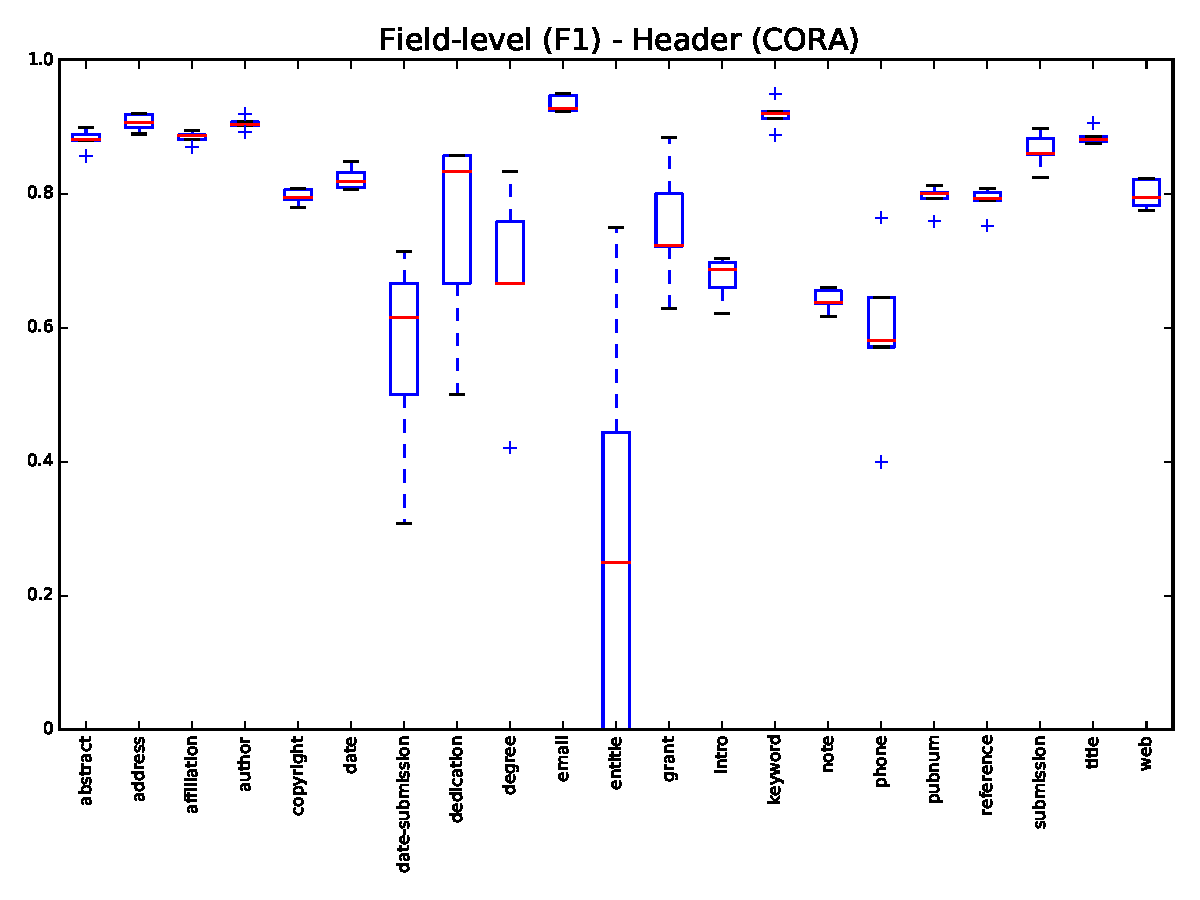
\includegraphics[width=0.75\textwidth]{../../figs/baseline/H_C/boxplot-field-level.pdf}}\\
%   \subfloat[][]{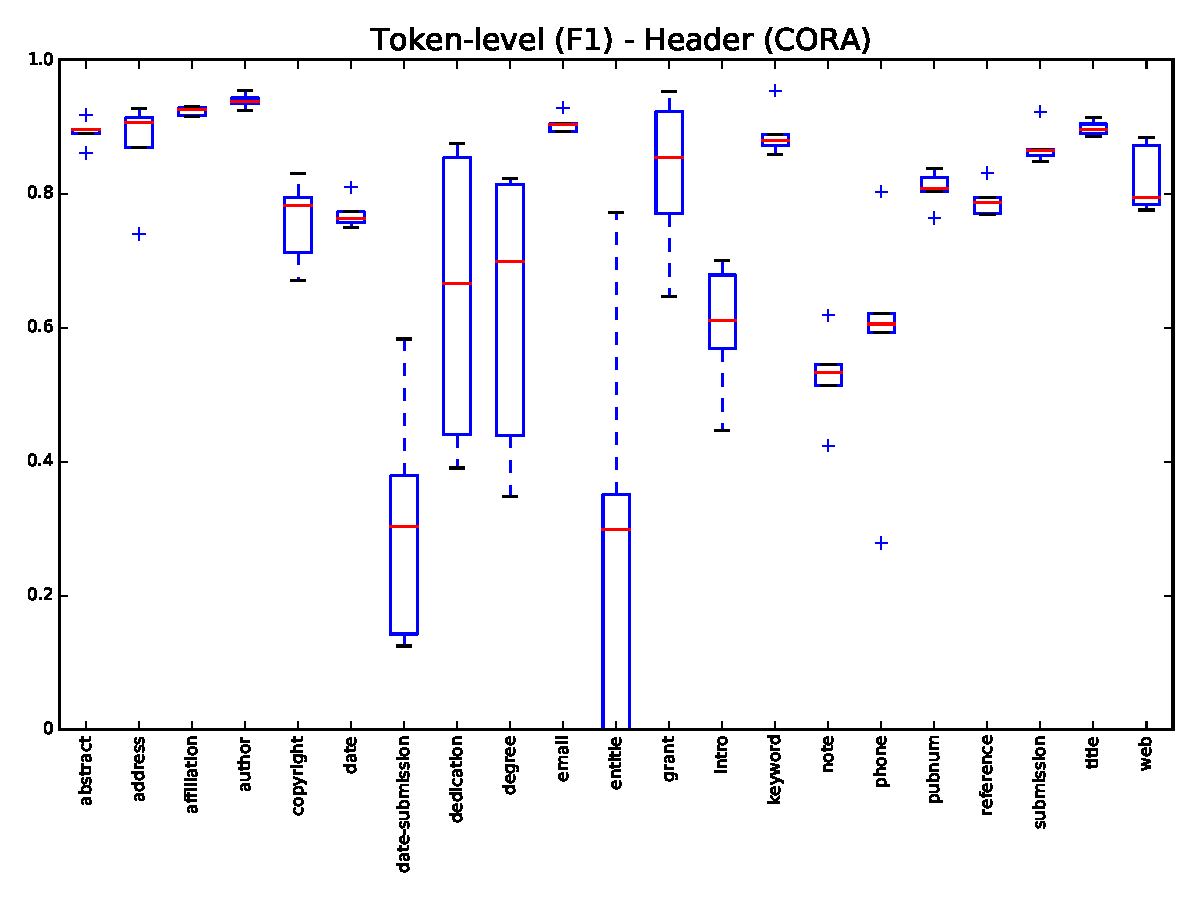
\includegraphics[width=0.75\textwidth]{../../figs/baseline/H_C/boxplot-token-level.pdf}}
% \end{figure}

% \begin{figure}[H]
%   \centering
%   \subfloat[][]{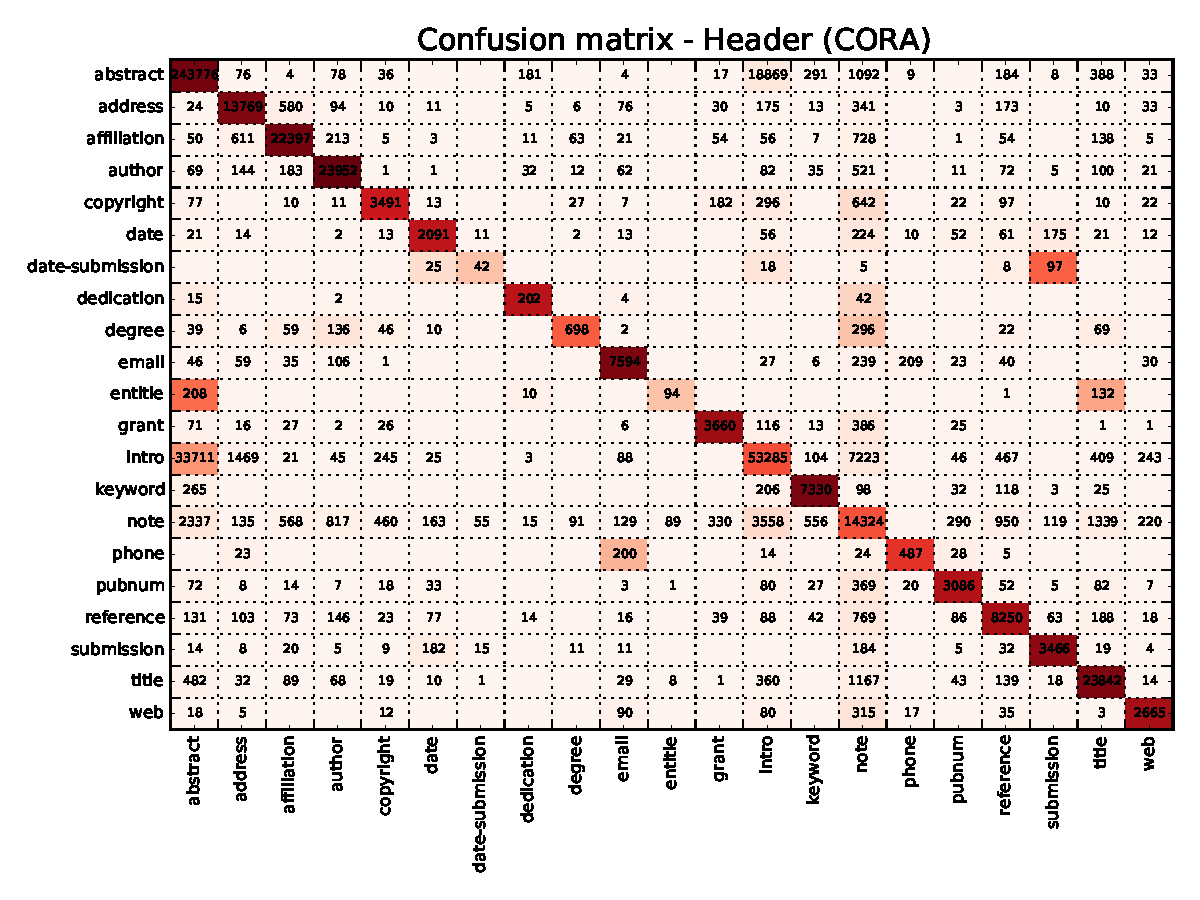
\includegraphics[width=0.75\textwidth]{../../figs/baseline/H_C/confusion_totals.pdf}}
% \end{figure}

% %%%%%%%%%%%%%%%%%%%%%%%%%%%%%%%%%%%%%%%%%%%%%%

% \subsubsection{Header model - Cora dataset appending HEP dataset}

% %%%%%%%%%%%%%%%%%%%%%%%%%%%%%%%%%%%%%%%%%%%%%%

% \begin{figure}[H]
%   \centering
%   \subfloat[][]{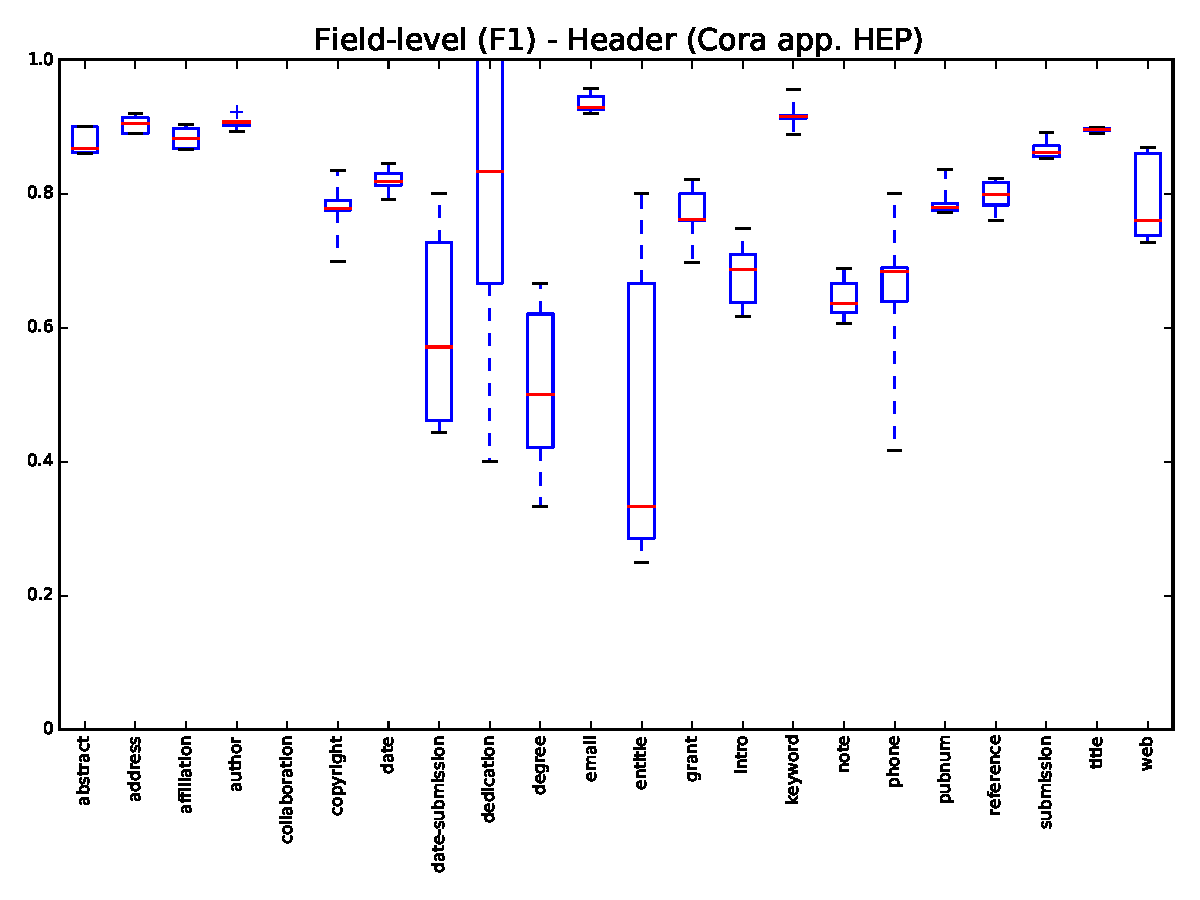
\includegraphics[width=0.75\textwidth]{../../figs/baseline/H_CappH/boxplot-field-level.pdf}}\\
%   \subfloat[][]{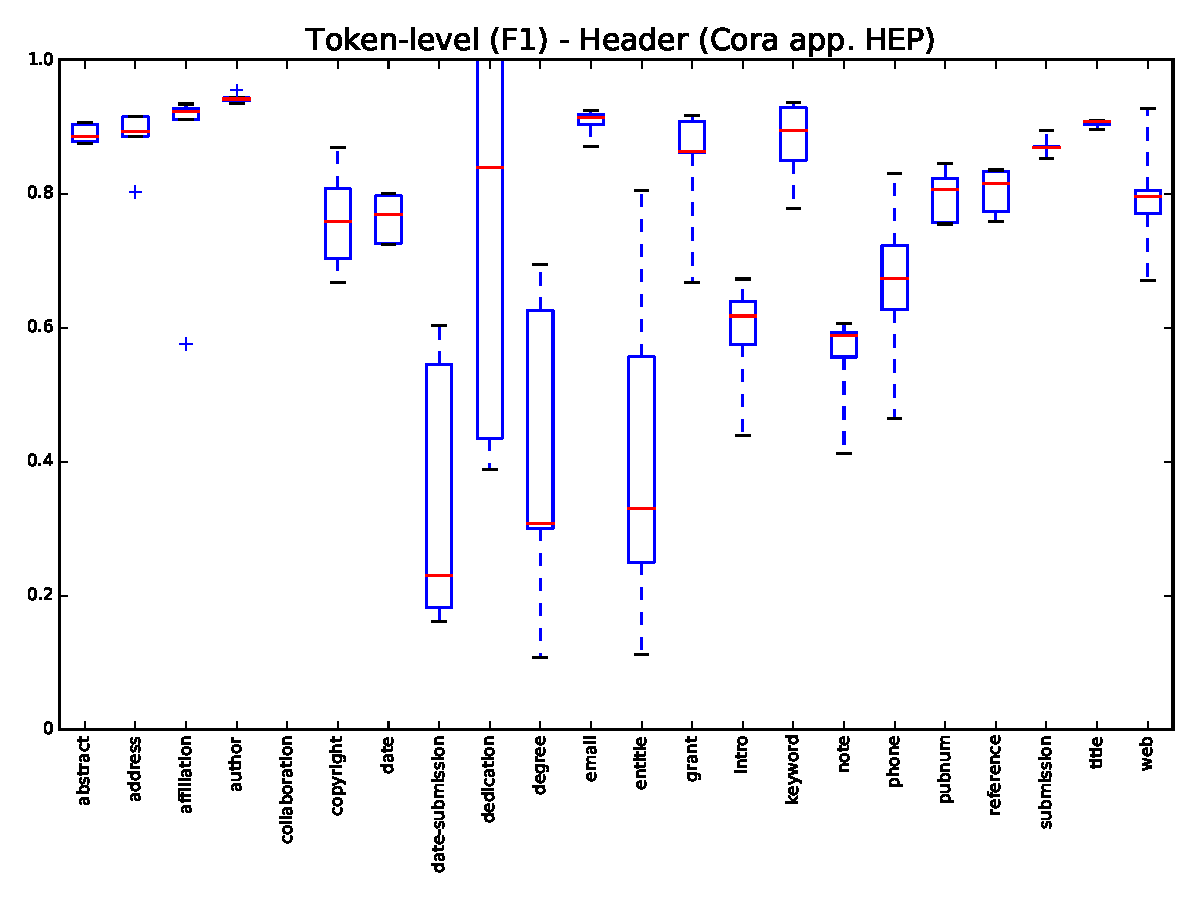
\includegraphics[width=0.75\textwidth]{../../figs/baseline/H_CappH/boxplot-token-level.pdf}}
% \end{figure}

% \begin{figure}[H]
%   \centering
%   \subfloat[][]{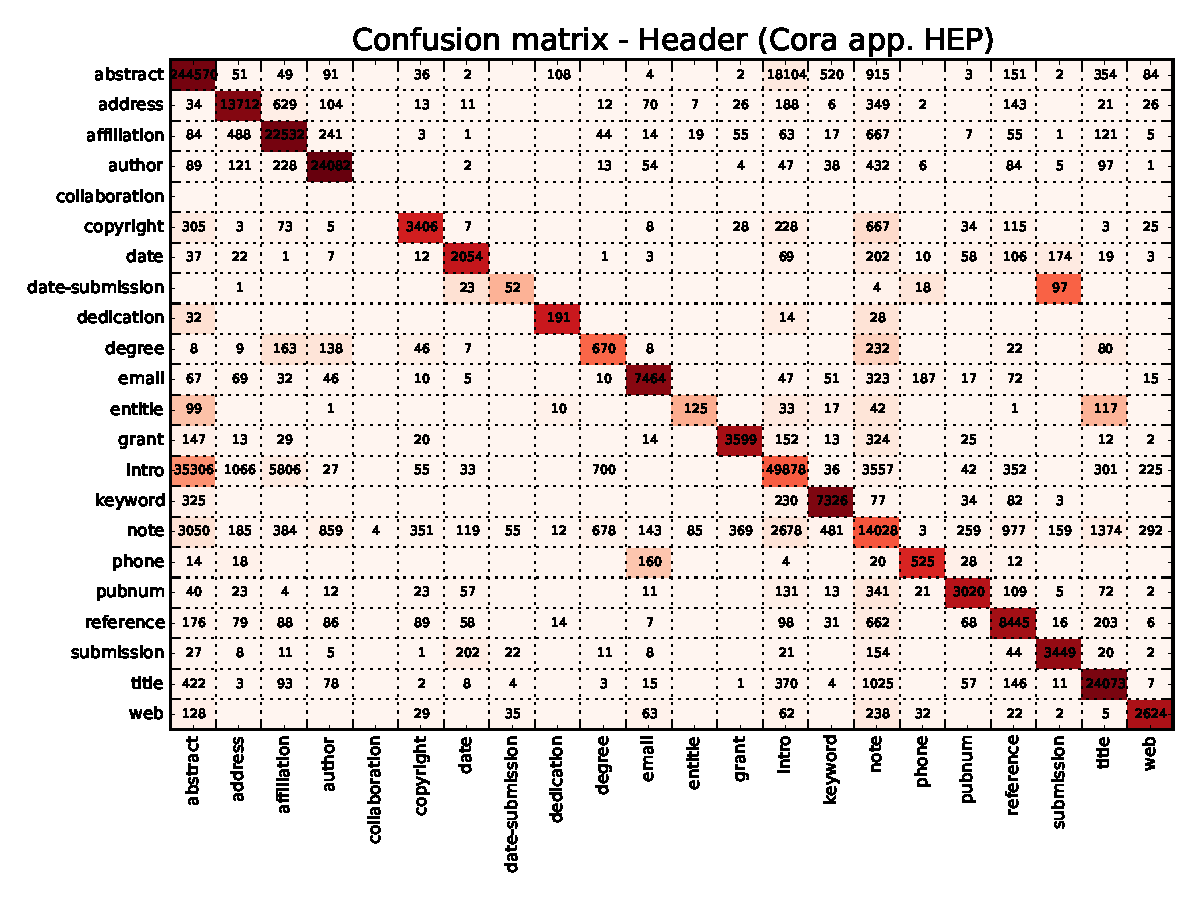
\includegraphics[width=0.75\textwidth]{../../figs/baseline/H_CappH/confusion_totals.pdf}}
% \end{figure}

% %%%%%%%%%%%%%%%%%%%%%%%%%%%%%%%%%%%%%%%%%%%%%%

% \subsubsection{Header model - Cora and HEP combined datasets}

% %%%%%%%%%%%%%%%%%%%%%%%%%%%%%%%%%%%%%%%%%%%%%%

% \begin{figure}[H]
%   \centering
%   \subfloat[][]{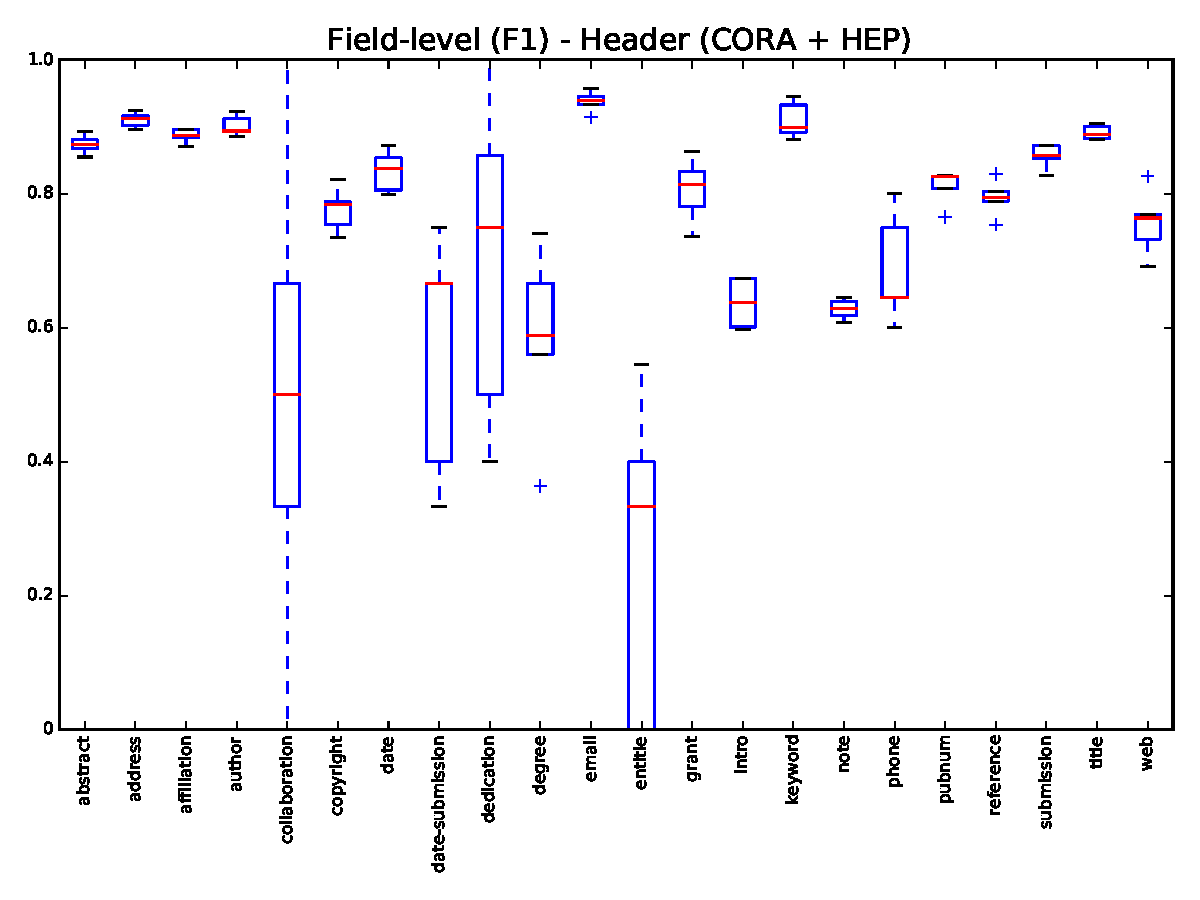
\includegraphics[width=0.75\textwidth]{../../figs/baseline/H_CH/boxplot-field-level.pdf}}\\
%   \subfloat[][]{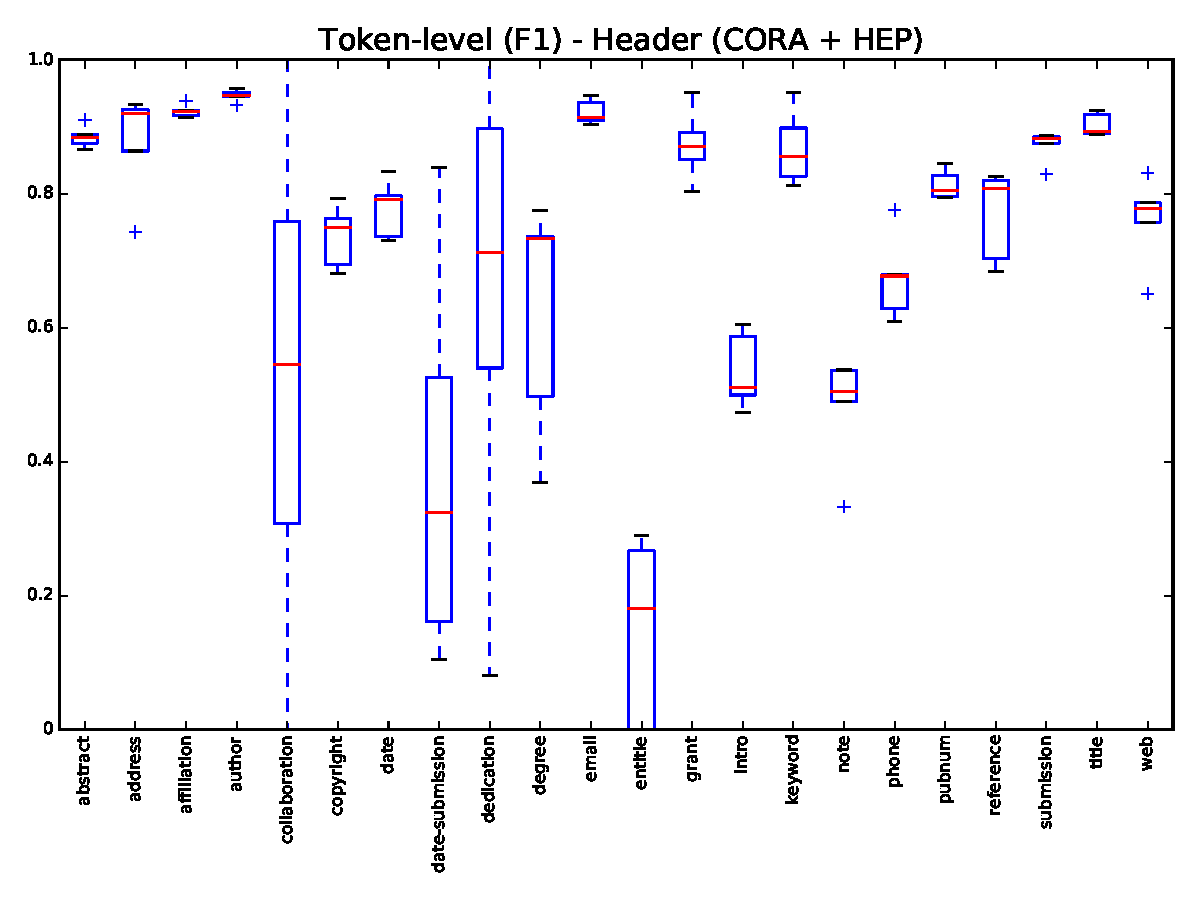
\includegraphics[width=0.75\textwidth]{../../figs/baseline/H_CH/boxplot-token-level.pdf}}
% \end{figure}

% \begin{figure}[H]
%   \centering
%   \subfloat[][]{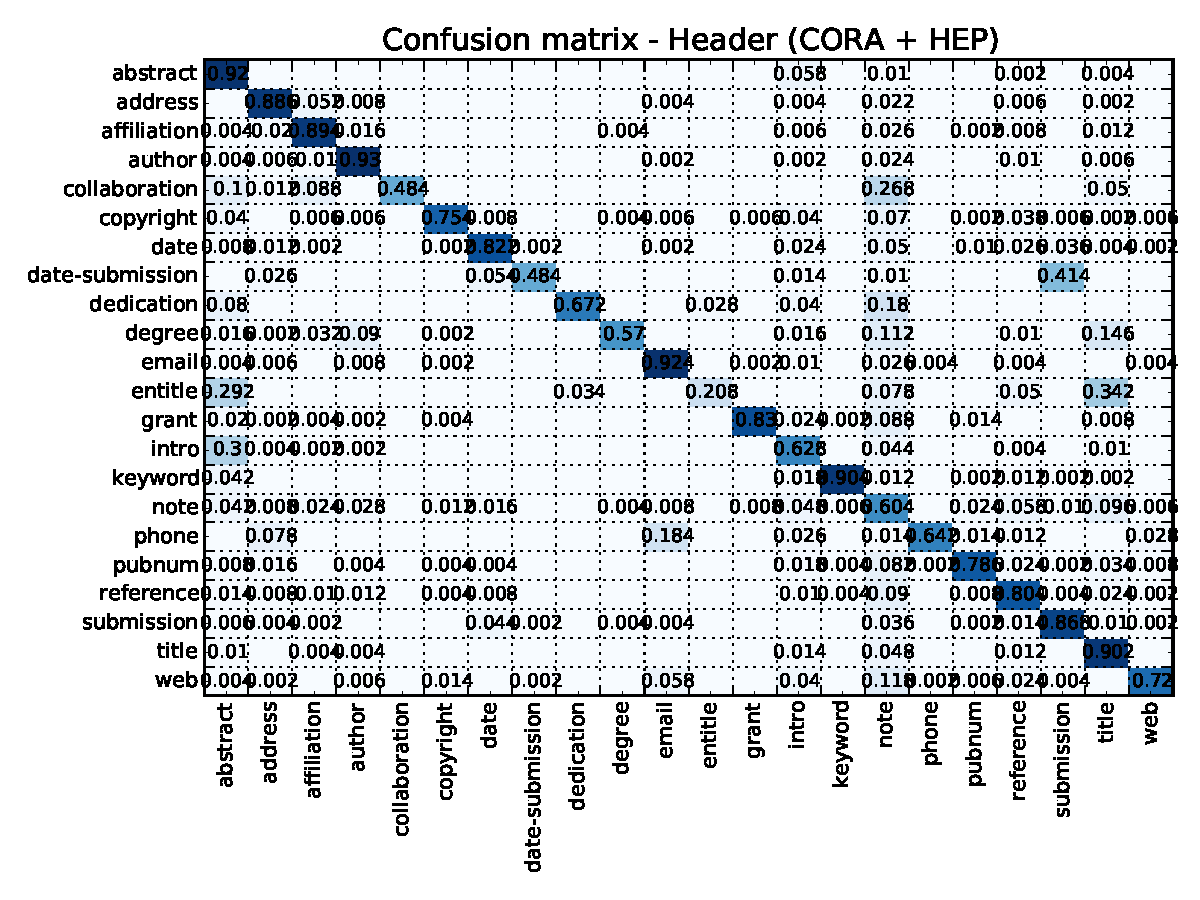
\includegraphics[width=0.75\textwidth]{../../figs/baseline/H_CH/confusion_averages.pdf}}\\
%   \subfloat[][]{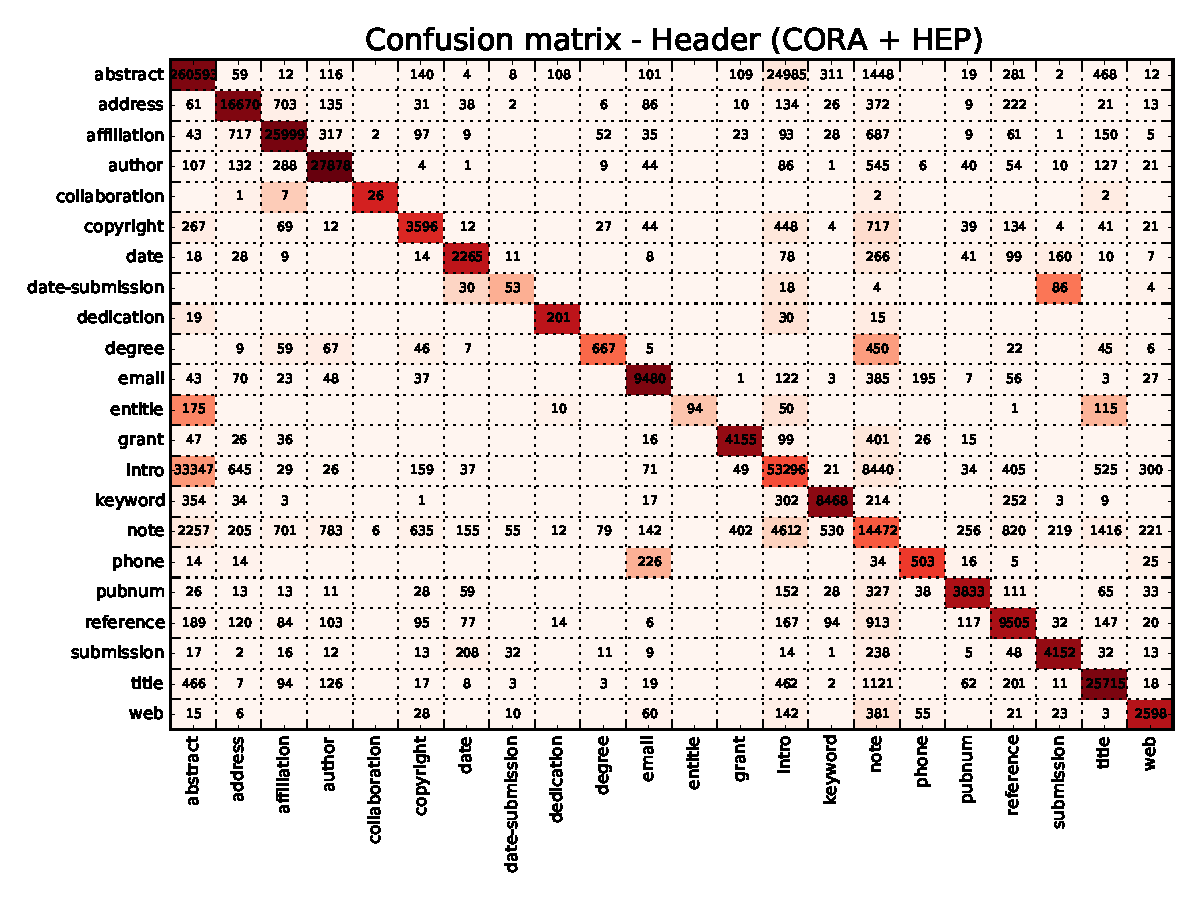
\includegraphics[width=0.75\textwidth]{../../figs/baseline/H_CH/confusion_totals.pdf}}
% \end{figure}

% %%%%%%%%%%%%%%%%%%%%%%%%%%%%%%%%%%%%%%%%%%%%%%

% \subsubsection{Header model - HEP dataset}

% %%%%%%%%%%%%%%%%%%%%%%%%%%%%%%%%%%%%%%%%%%%%%%

% \begin{figure}[H]
%   \centering
%   \subfloat[][]{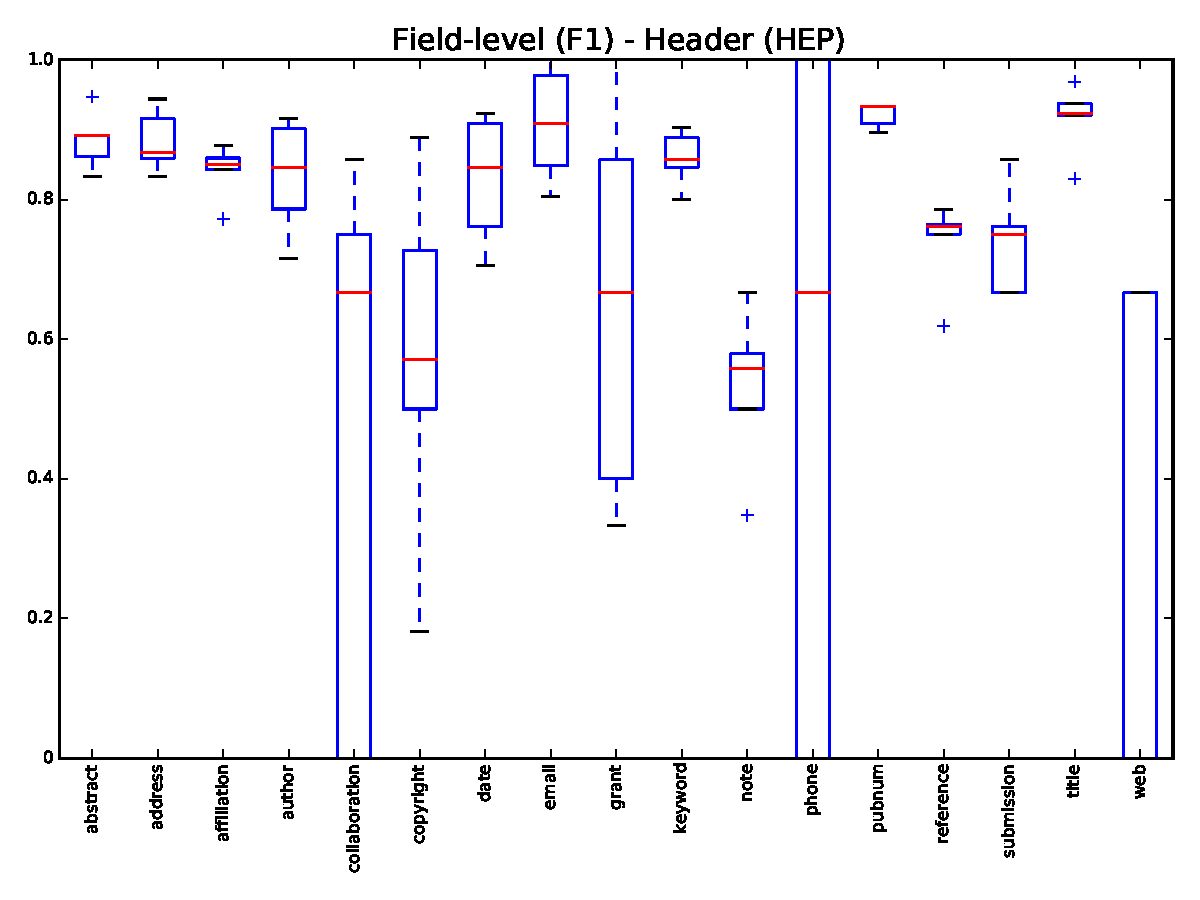
\includegraphics[width=0.75\textwidth]{../../figs/baseline/H_H/boxplot-field-level.pdf}}\\
%   \subfloat[][]{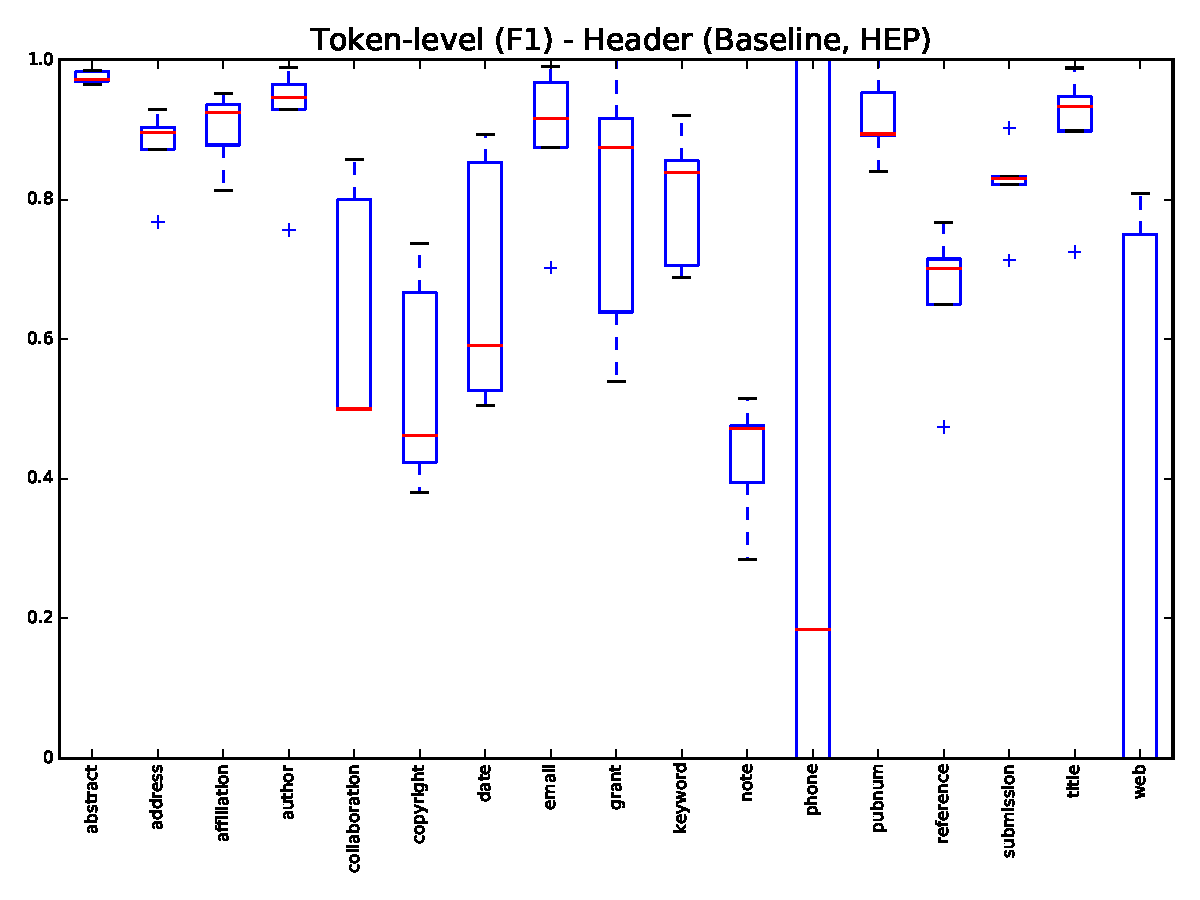
\includegraphics[width=0.75\textwidth]{../../figs/baseline/H_H/boxplot-token-level.pdf}}
% \end{figure}

% \begin{figure}[H]
%   \centering
%   \subfloat[][]{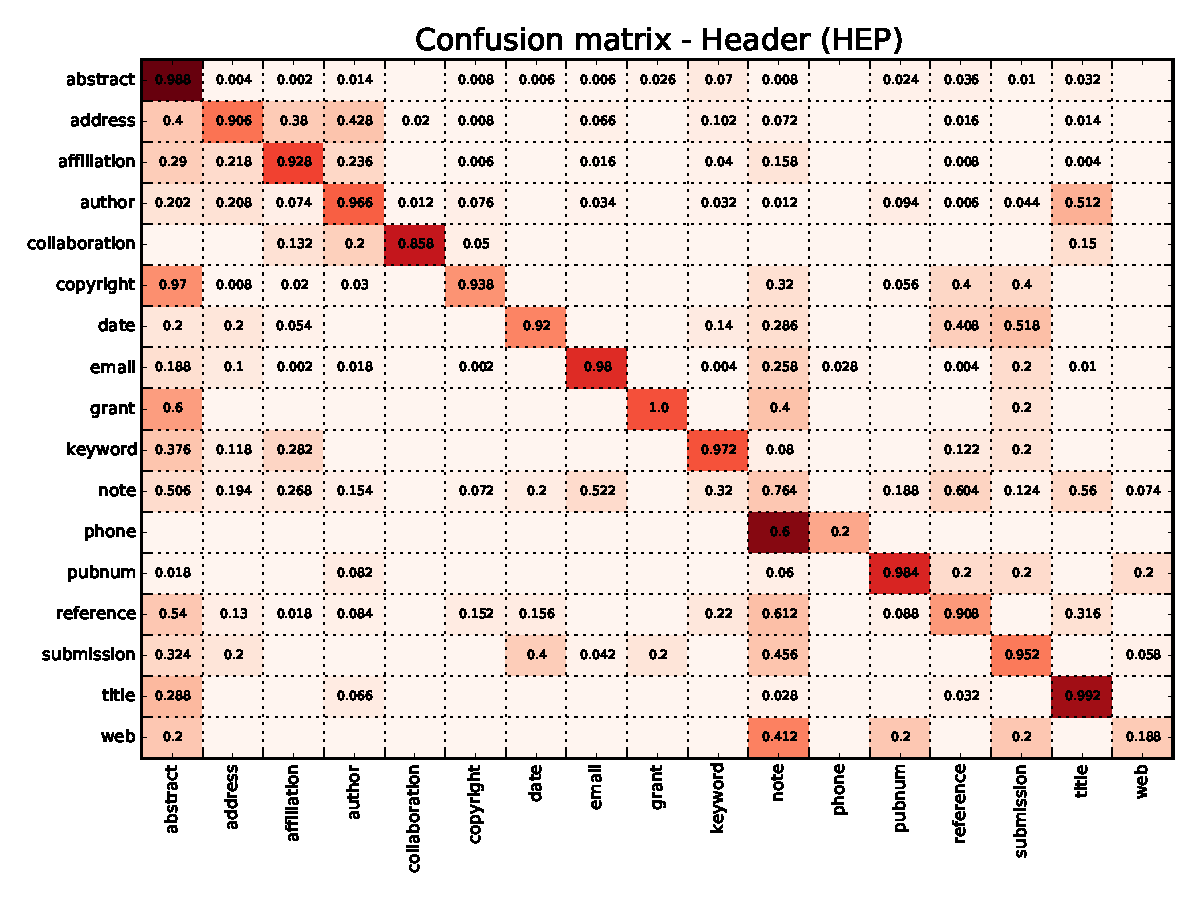
\includegraphics[width=0.75\textwidth]{../../figs/baseline/H_H/confusion_averages.pdf}}\\
%   \subfloat[][]{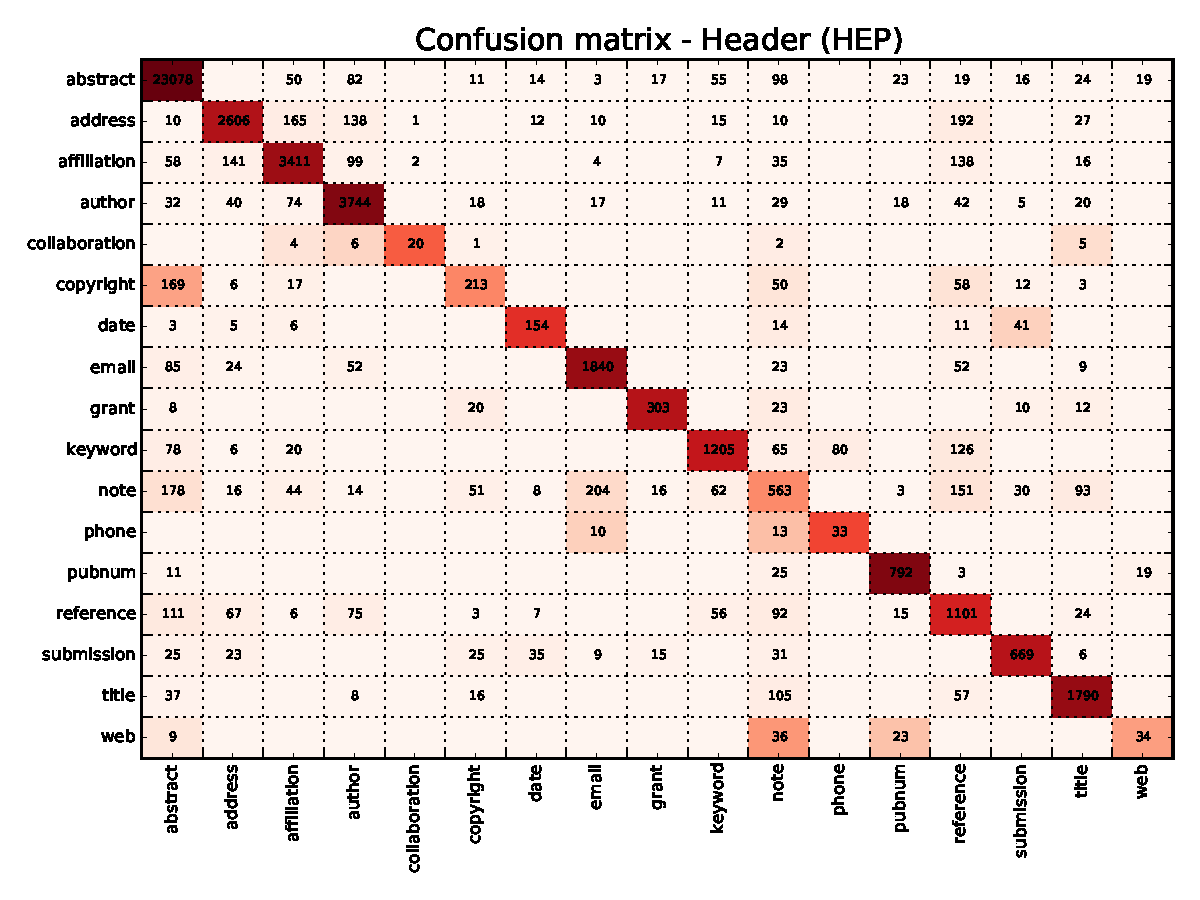
\includegraphics[width=0.75\textwidth]{../../figs/baseline/H_H/confusion_totals.pdf}}
% \end{figure}

% %%%%%%%%%%%%%%%%%%%%%%%%%%%%%%%%%%%%%%%%%%%%%%

% \subsubsection{Header model - HEP dataset appending CORA dataset}

% %%%%%%%%%%%%%%%%%%%%%%%%%%%%%%%%%%%%%%%%%%%%%%

% \begin{figure}[H]
%   \centering
%   \subfloat[][]{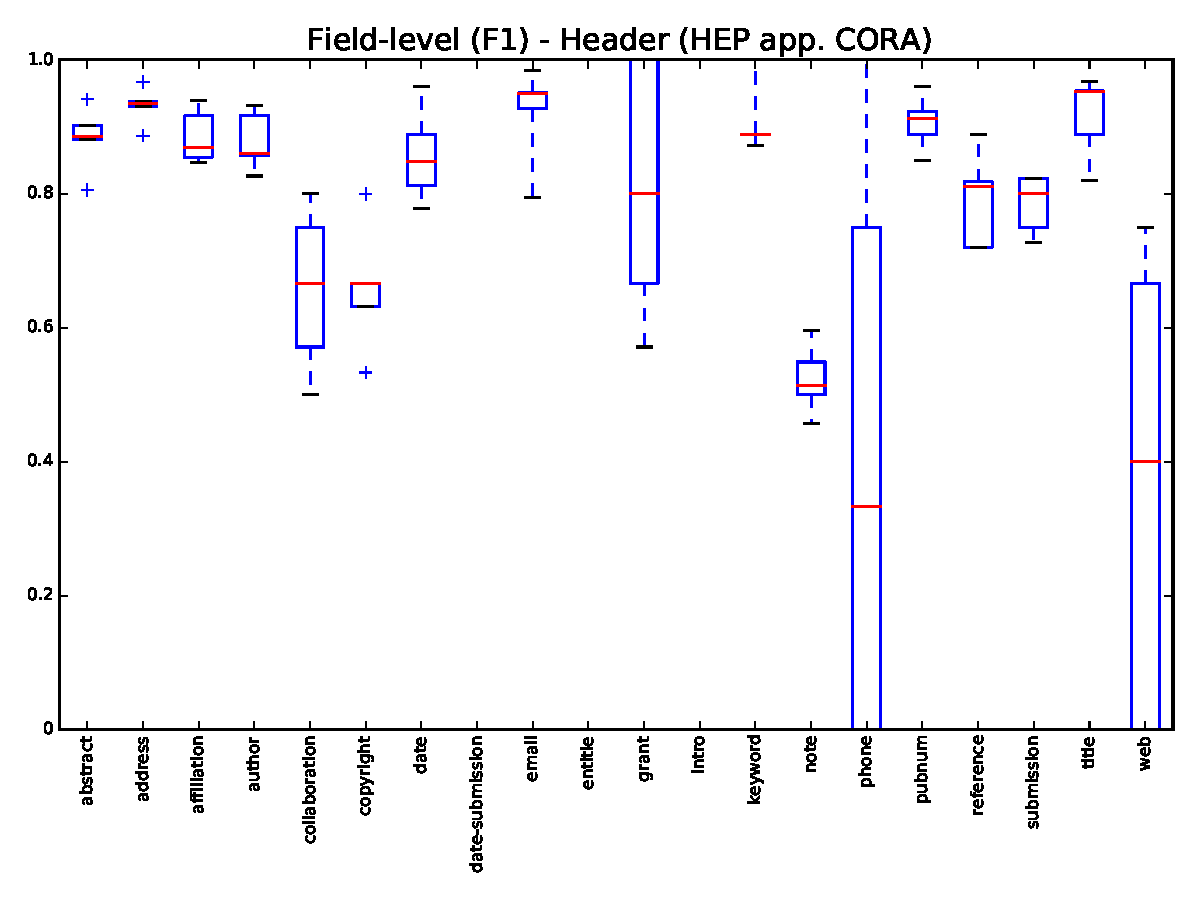
\includegraphics[width=0.75\textwidth]{../../figs/baseline/H_HappC/boxplot-field-level.pdf}}\\
%   \subfloat[][]{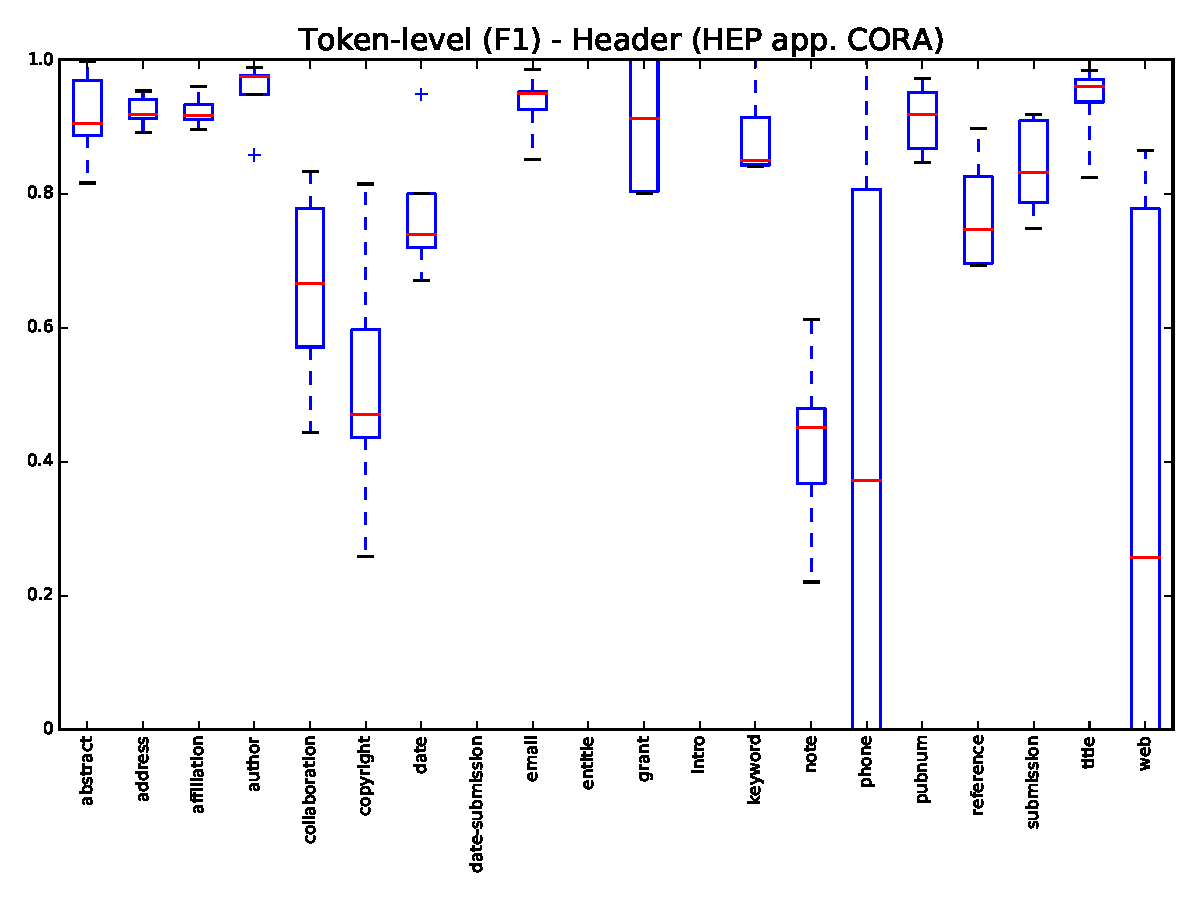
\includegraphics[width=0.75\textwidth]{../../figs/baseline/H_HappC/boxplot-token-level.pdf}}
% \end{figure}

% \begin{figure}[H]
%   \centering
%   \subfloat[][]{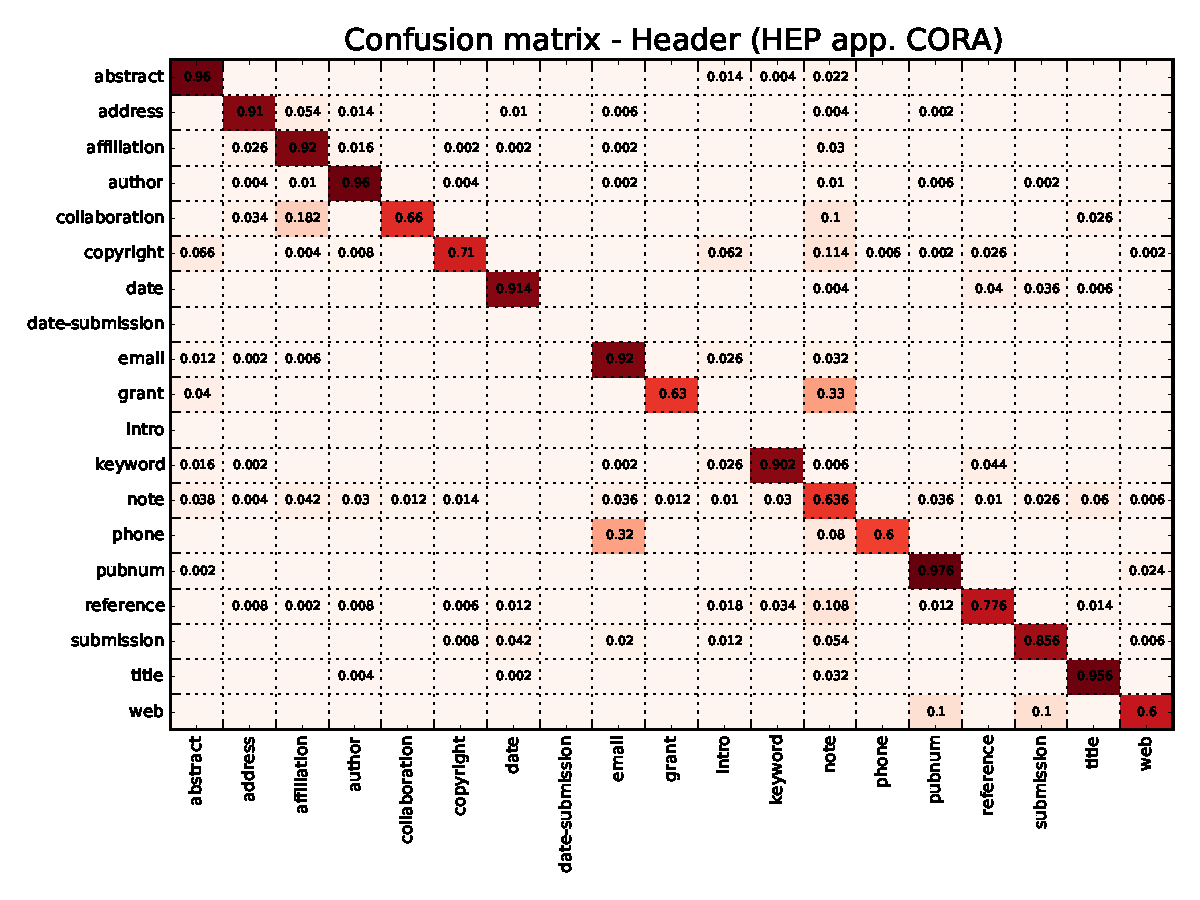
\includegraphics[width=0.75\textwidth]{../../figs/baseline/H_HappC/confusion_averages.pdf}}\\
%   \subfloat[][]{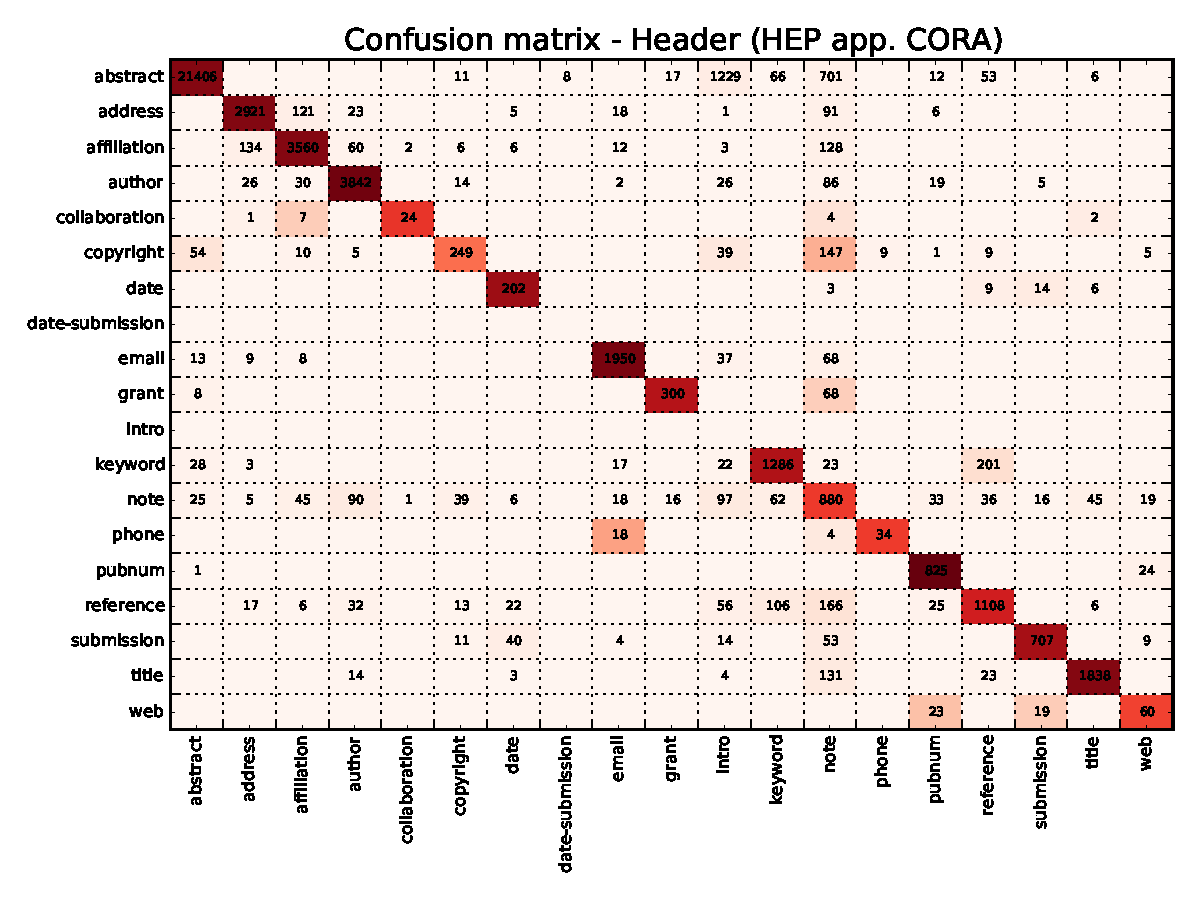
\includegraphics[width=0.75\textwidth]{../../figs/baseline/H_HappC/confusion_totals.pdf}}
% \end{figure}

% %%%%%%%%%%%%%%%%%%%%%%%%%%%%%%%%%%%%%%%%%%%%%%

% \subsubsection{Header model - HEP dataset appending 1/3 CORA dataset}

% %%%%%%%%%%%%%%%%%%%%%%%%%%%%%%%%%%%%%%%%%%%%%%

% \begin{figure}[H]
%   \centering
%   \subfloat[][]{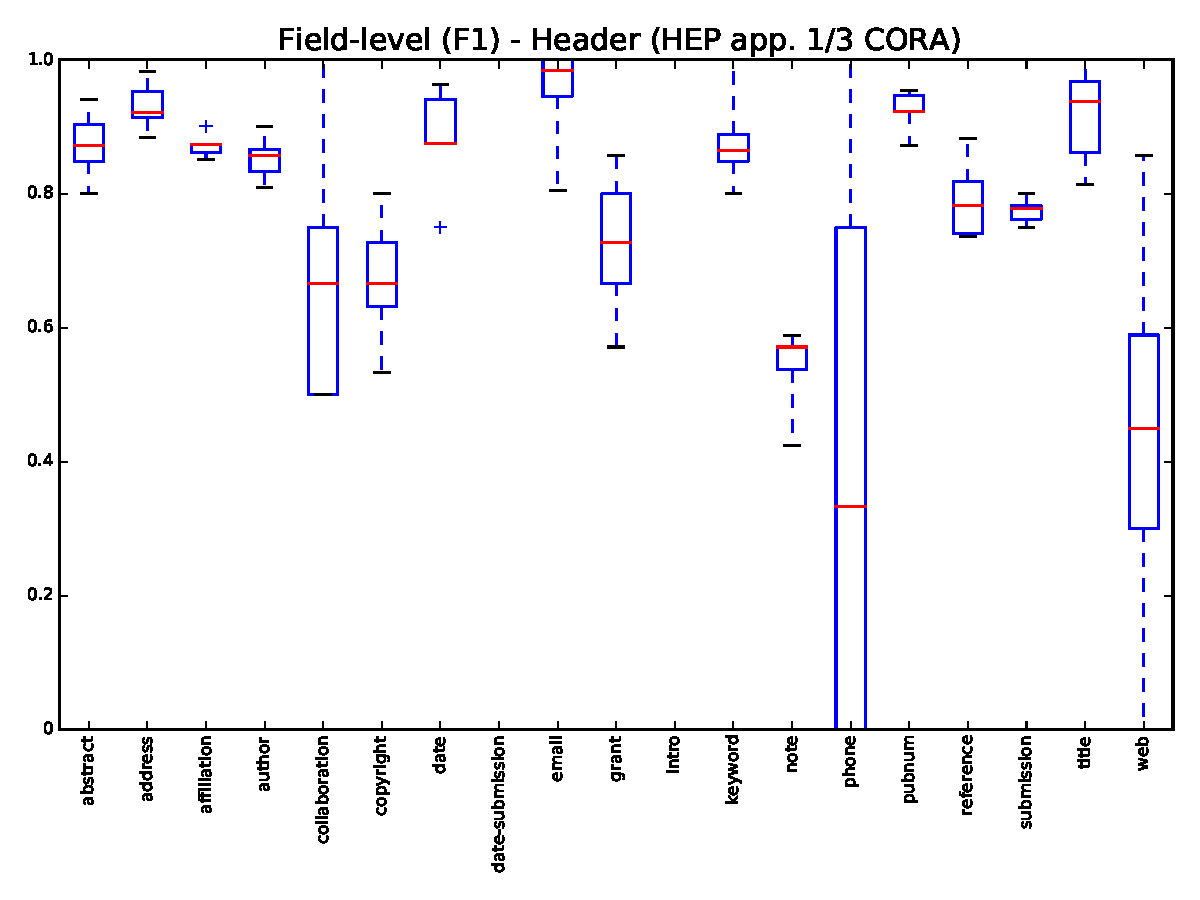
\includegraphics[width=0.75\textwidth]{../../figs/baseline/H_HappC333/boxplot-field-level.pdf}}\\
%   \subfloat[][]{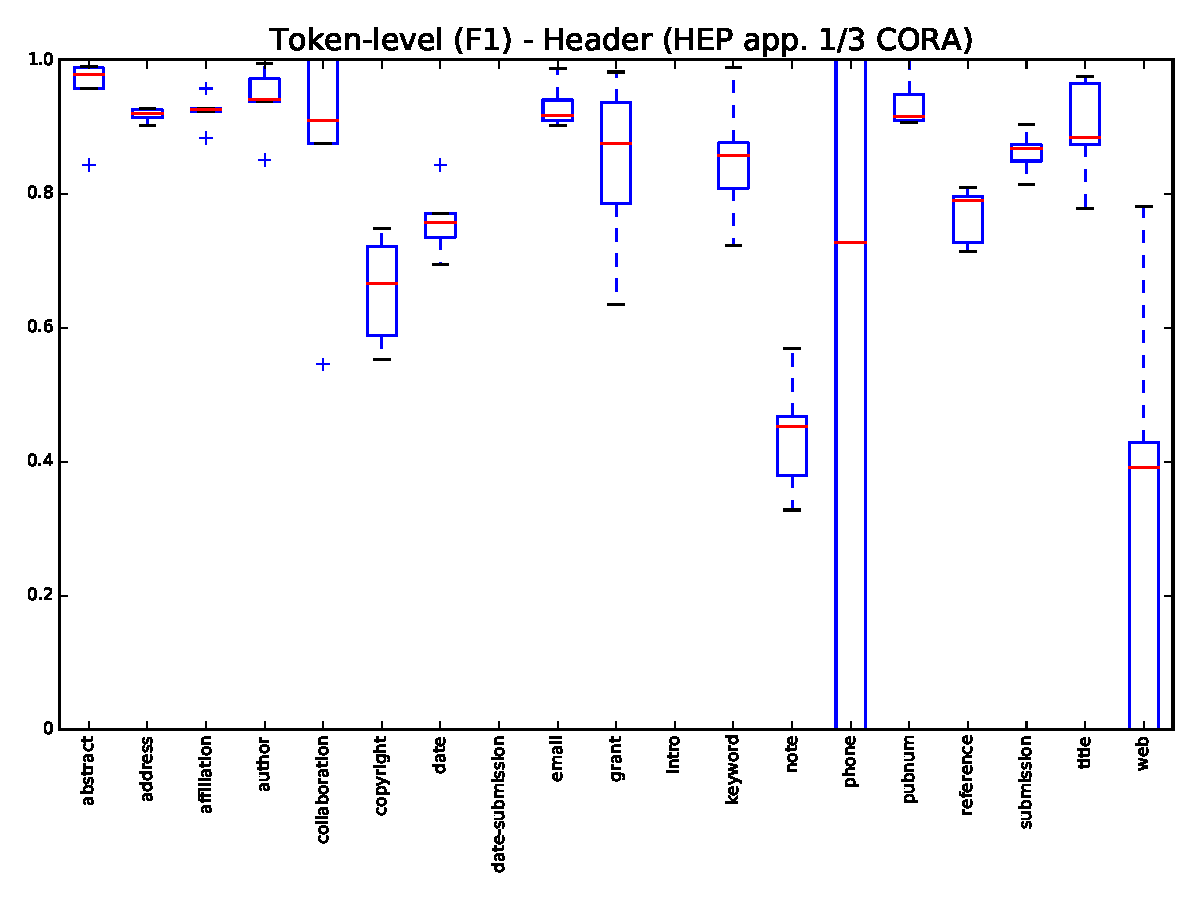
\includegraphics[width=0.75\textwidth]{../../figs/baseline/H_HappC333/boxplot-token-level.pdf}}
% \end{figure}

% \begin{figure}[H]
%   \centering
%   \subfloat[][]{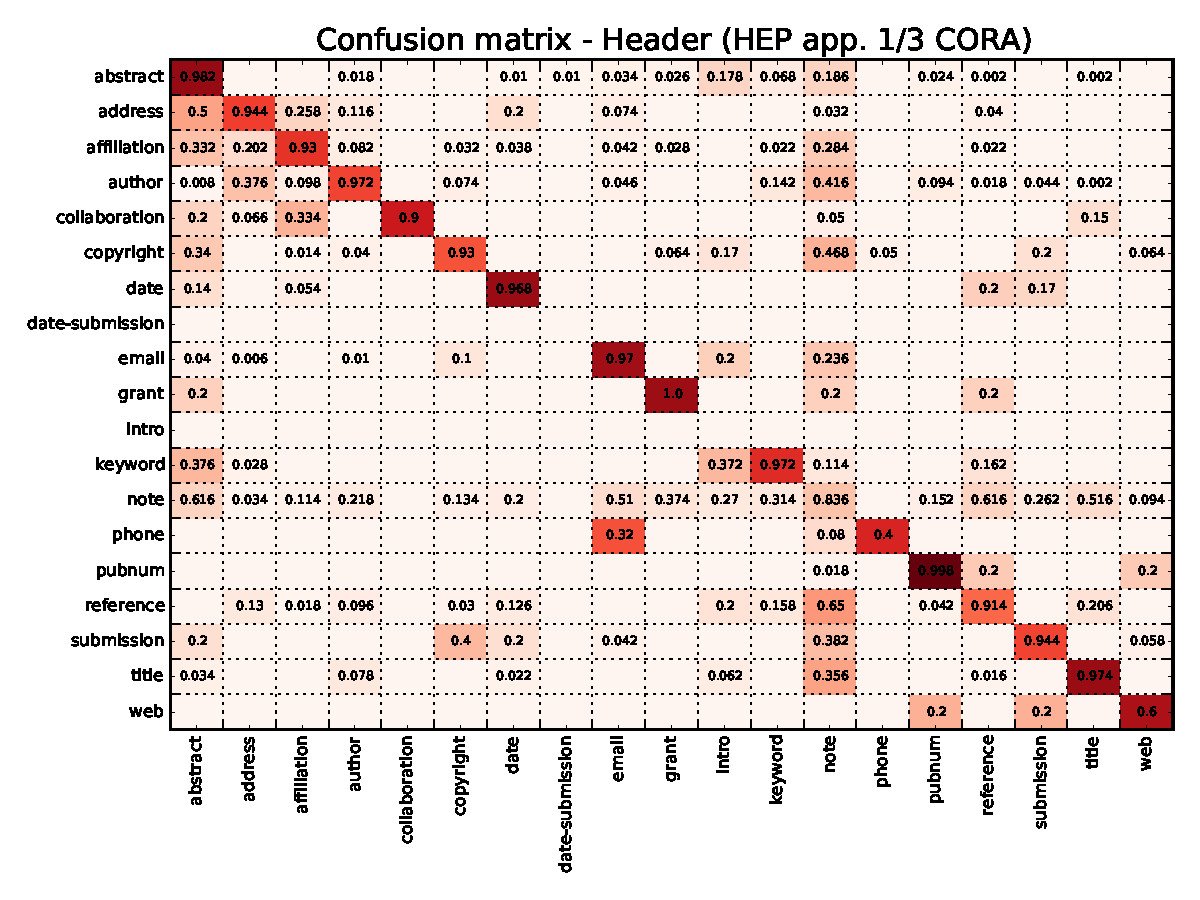
\includegraphics[width=0.75\textwidth]{../../figs/baseline/H_HappC333/confusion_averages.pdf}}\\
%   \subfloat[][]{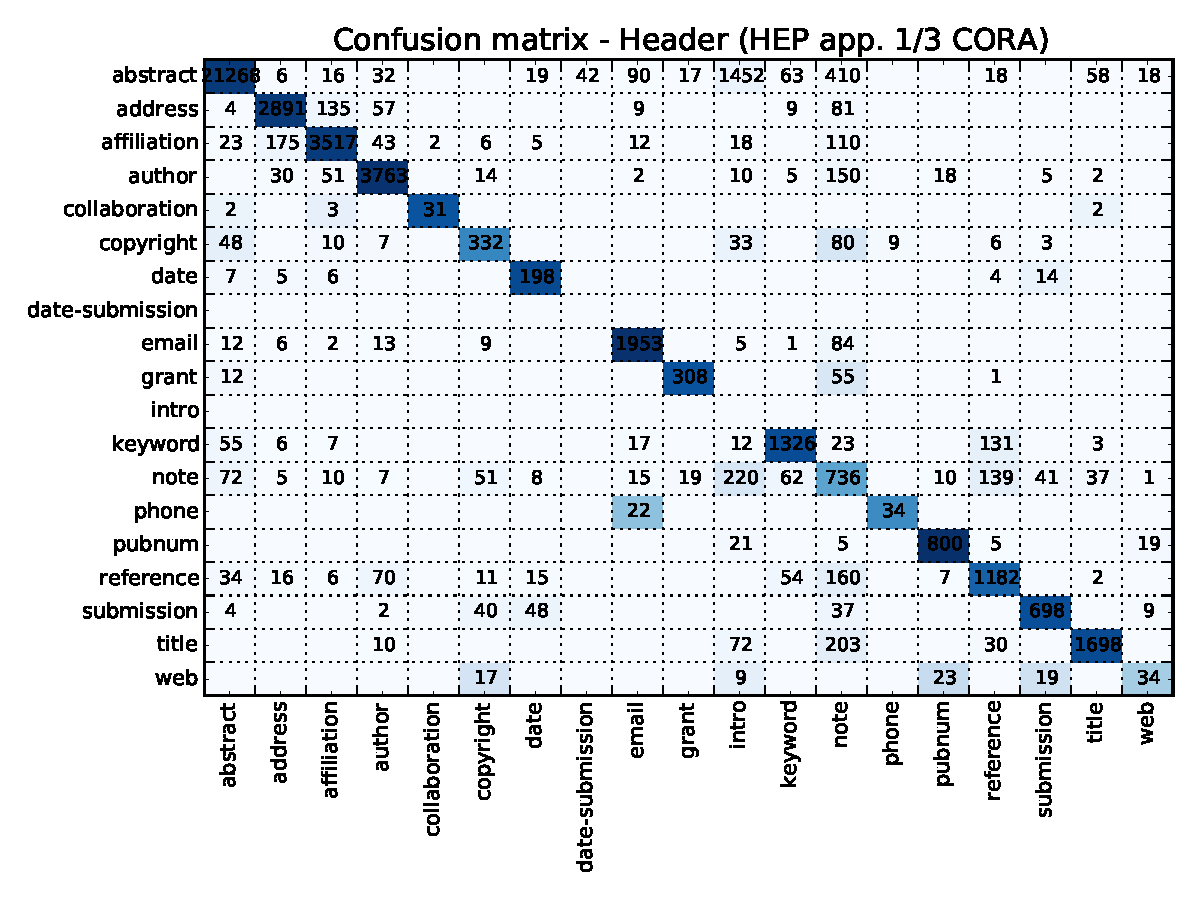
\includegraphics[width=0.75\textwidth]{../../figs/baseline/H_HappC333/confusion_totals.pdf}}
% \end{figure}

% %%%%%%%%%%%%%%%%%%%%%%%%%%%%%%%%%%%%%%%%%%%%%%

% \subsubsection{Header model - HEP dataset appending 2/3 CORA dataset}

% %%%%%%%%%%%%%%%%%%%%%%%%%%%%%%%%%%%%%%%%%%%%%%

% \begin{figure}[H]
%   \centering
%   \subfloat[][]{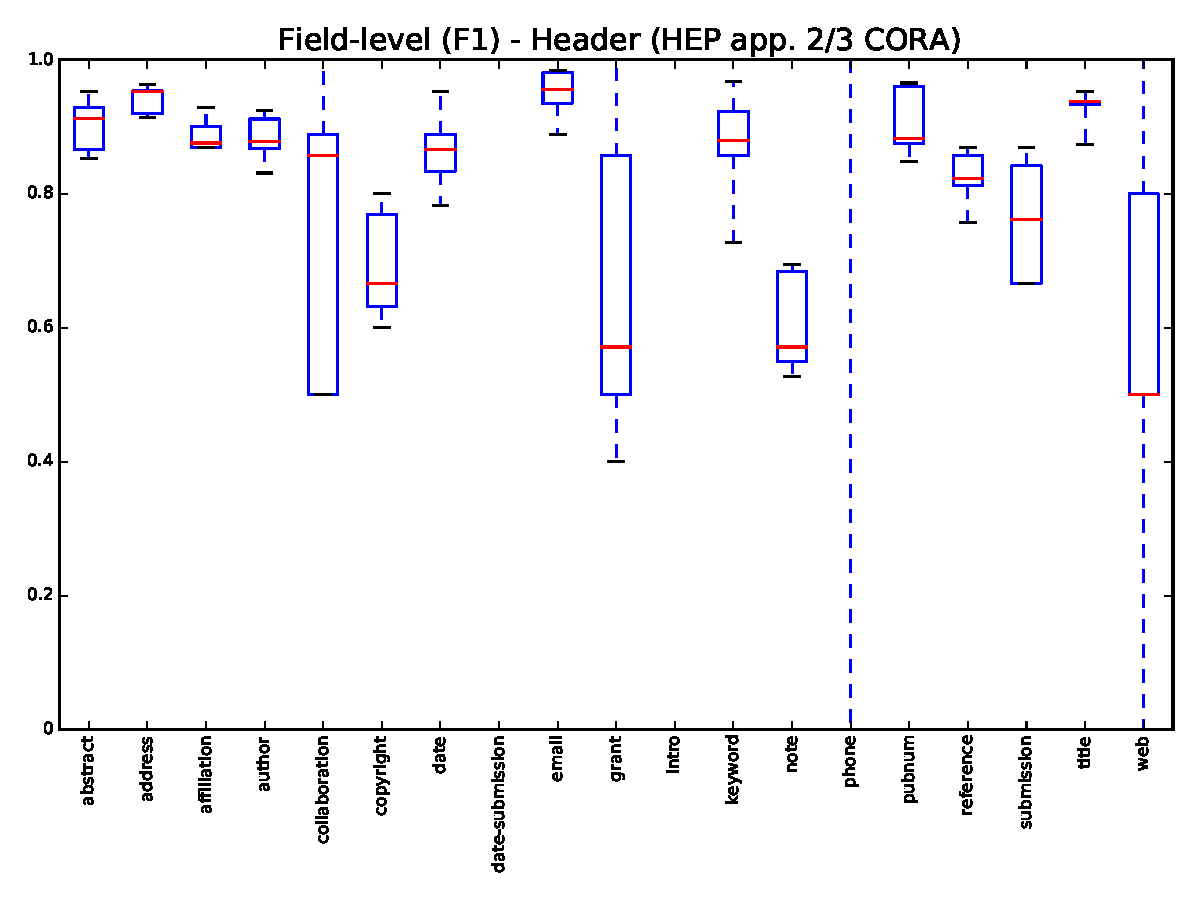
\includegraphics[width=0.75\textwidth]{../../figs/baseline/H_HappC666/boxplot-field-level.pdf}}\\
%   \subfloat[][]{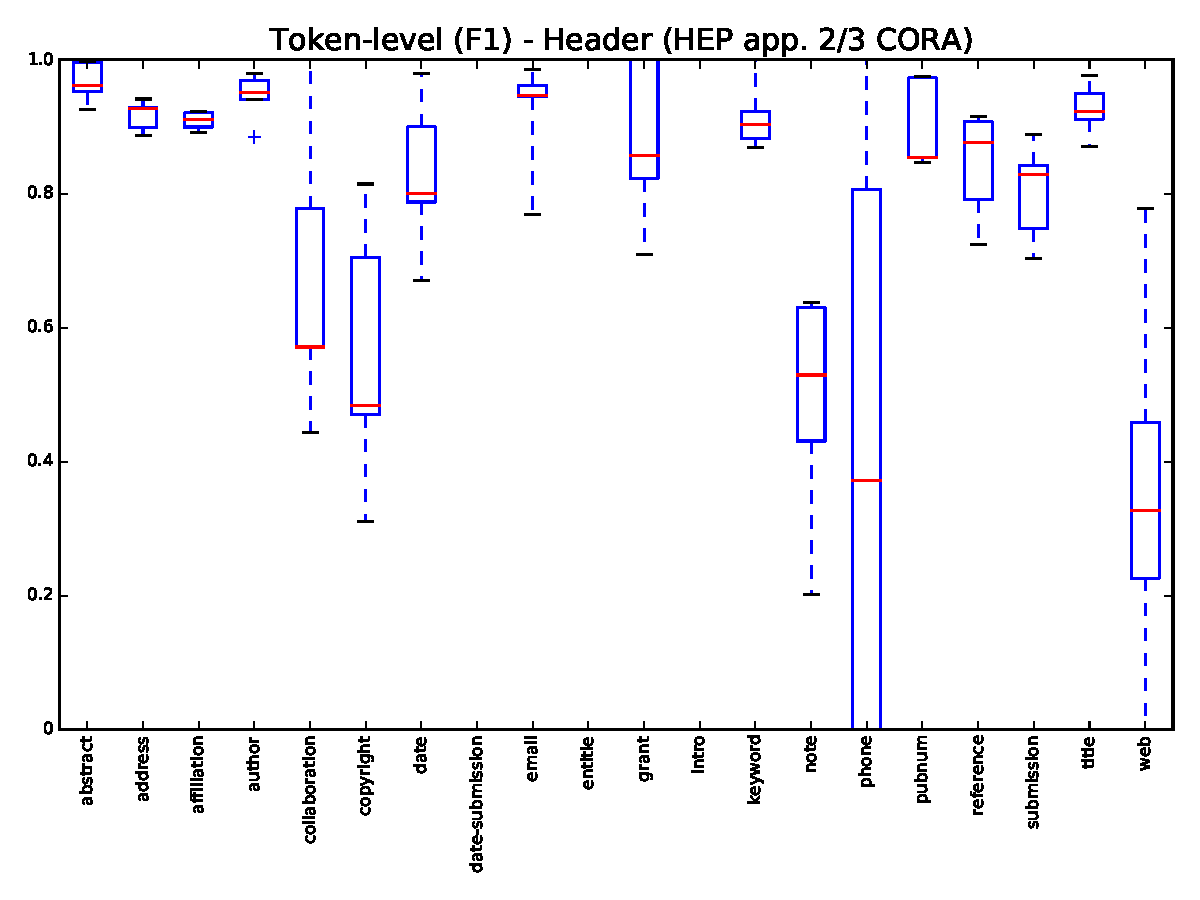
\includegraphics[width=0.75\textwidth]{../../figs/baseline/H_HappC666/boxplot-token-level.pdf}}
% \end{figure}

% \begin{figure}[H]
%   \centering
%   \subfloat[][]{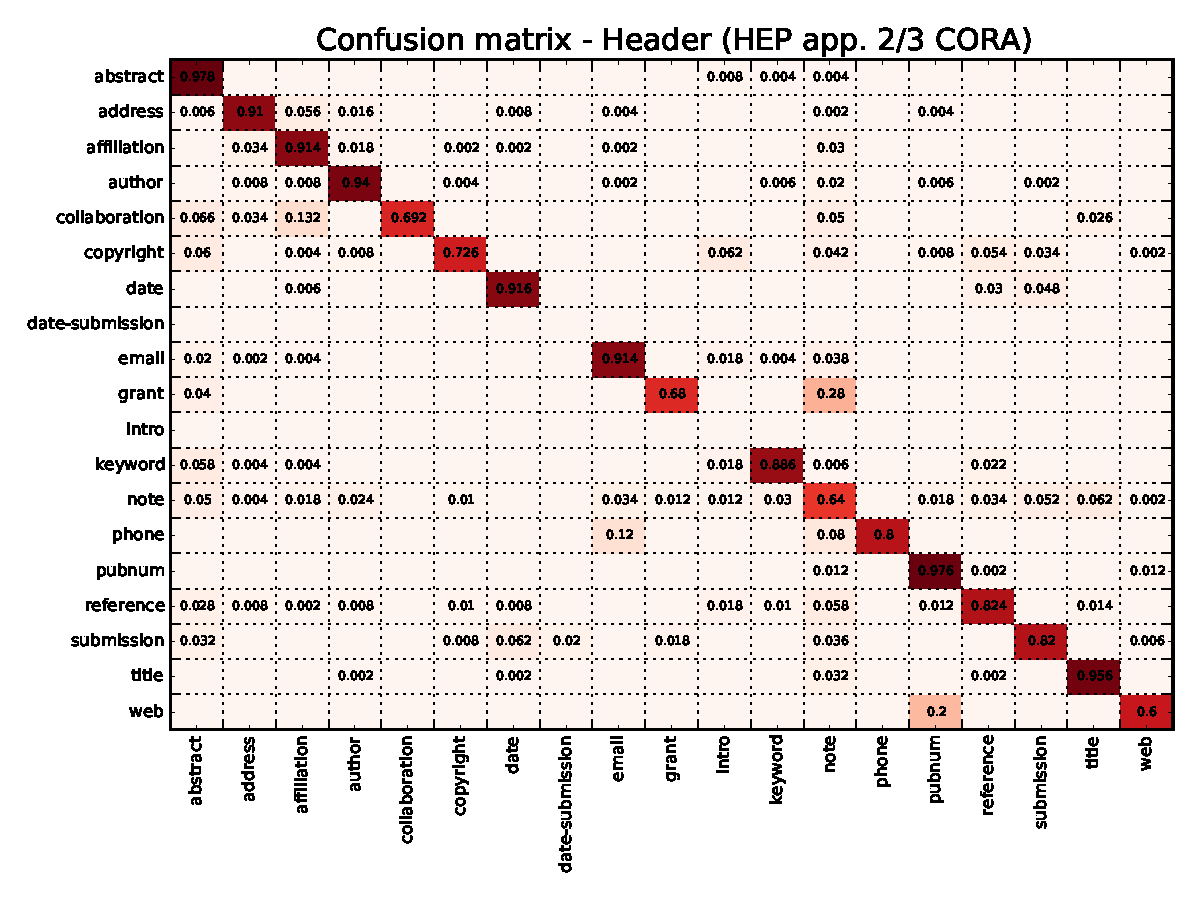
\includegraphics[width=0.75\textwidth]{../../figs/baseline/H_HappC666/confusion_averages.pdf}}\\
%   \subfloat[][]{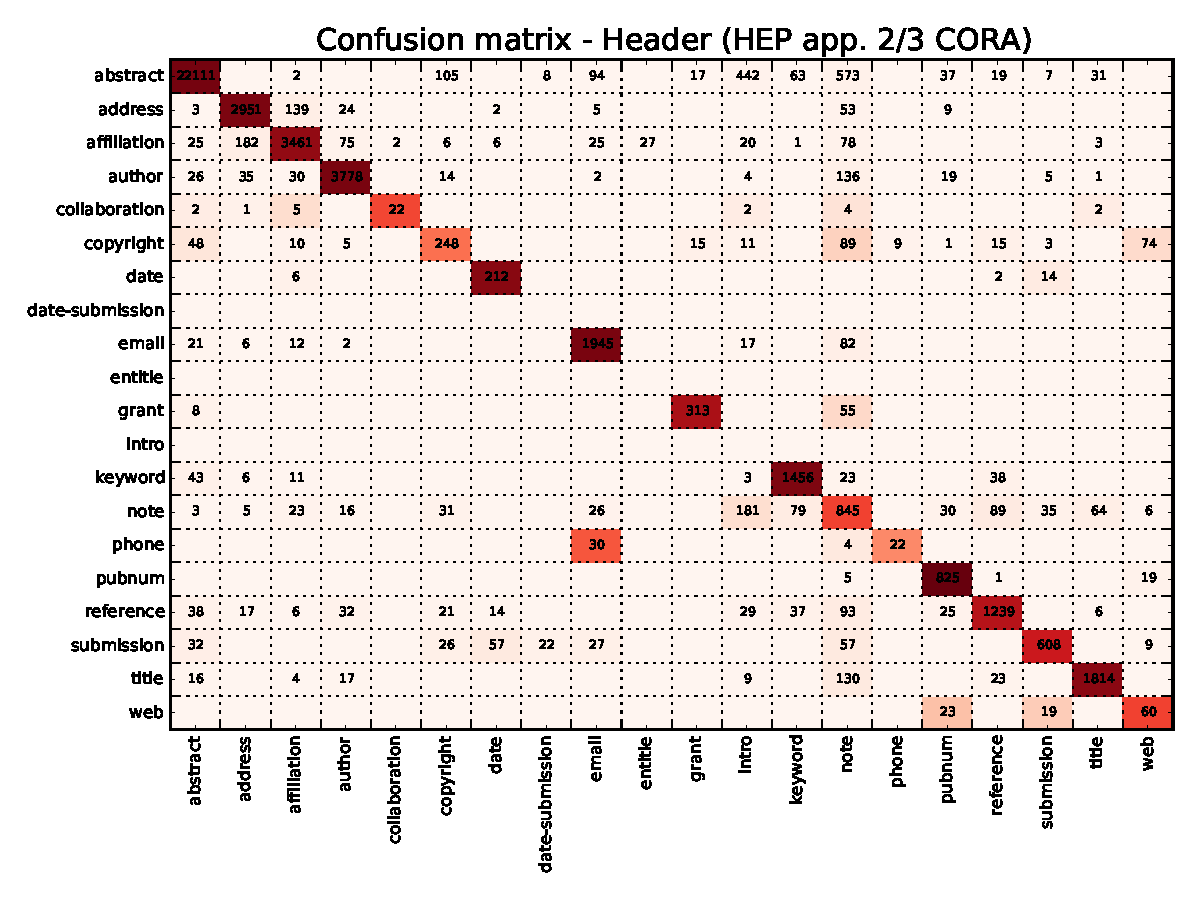
\includegraphics[width=0.75\textwidth]{../../figs/baseline/H_HappC666/confusion_totals.pdf}}
% \end{figure}

% %%%%%%%%%%%%%%%%%%%%%%%%%%%%%%%%%%%%%%%%%%%%%%

% \subsubsection{Segmentation model - Cora dataset}

% %%%%%%%%%%%%%%%%%%%%%%%%%%%%%%%%%%%%%%%%%%%%%%

% \begin{figure}[H]
%   \centering
%   \subfloat[][]{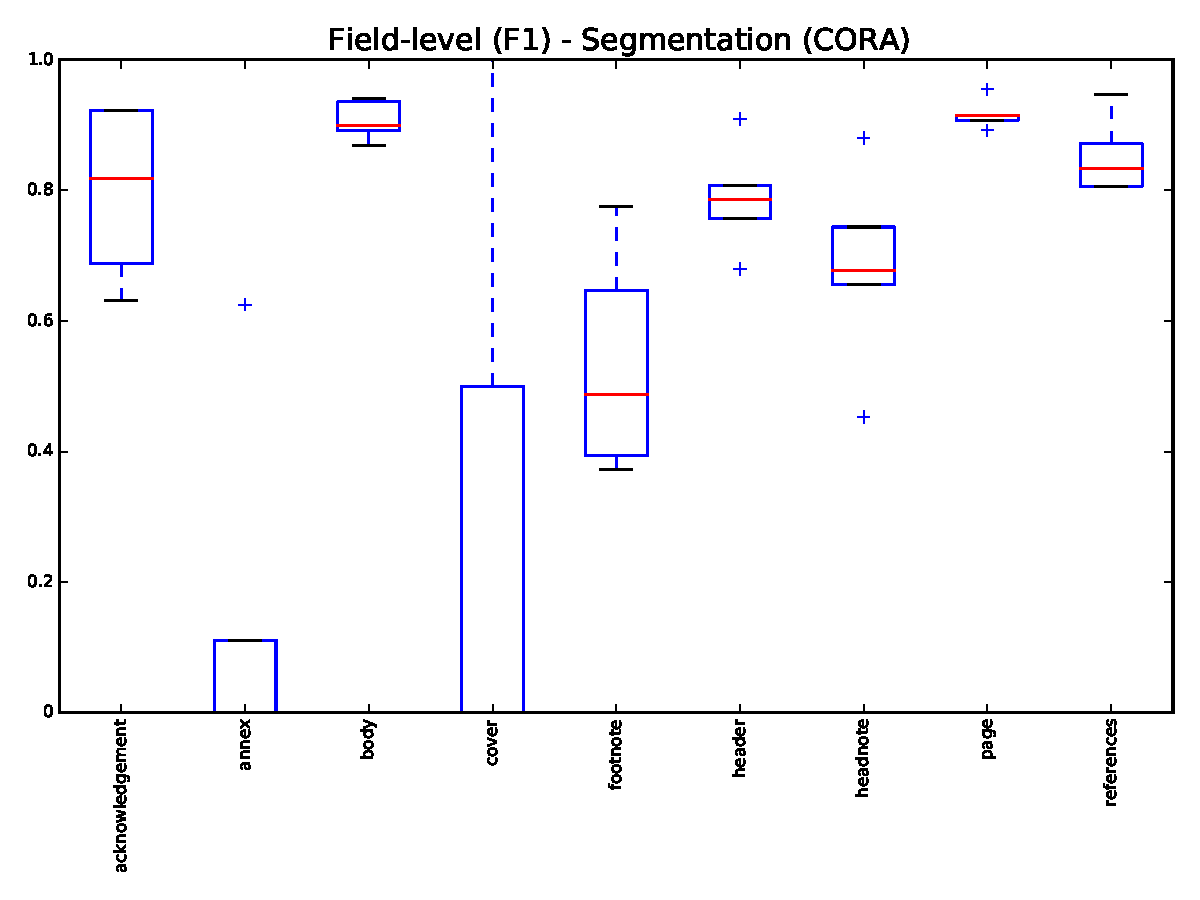
\includegraphics[width=0.75\textwidth]{../../figs/baseline/S_C/boxplot-field-level.pdf}}\\
%   \subfloat[][]{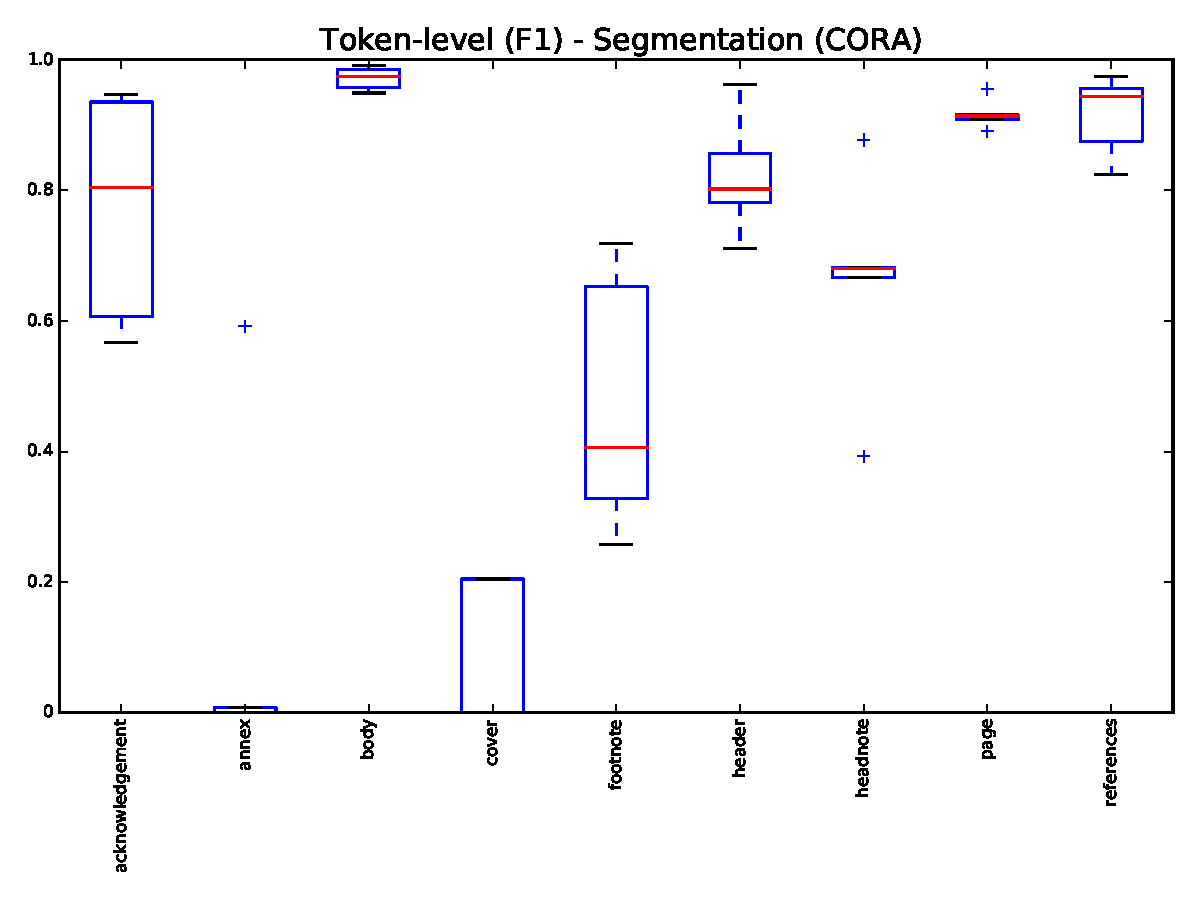
\includegraphics[width=0.75\textwidth]{../../figs/baseline/S_C/boxplot-token-level.pdf}}
% \end{figure}

% \begin{figure}[H]
%   \centering
%   \subfloat[][]{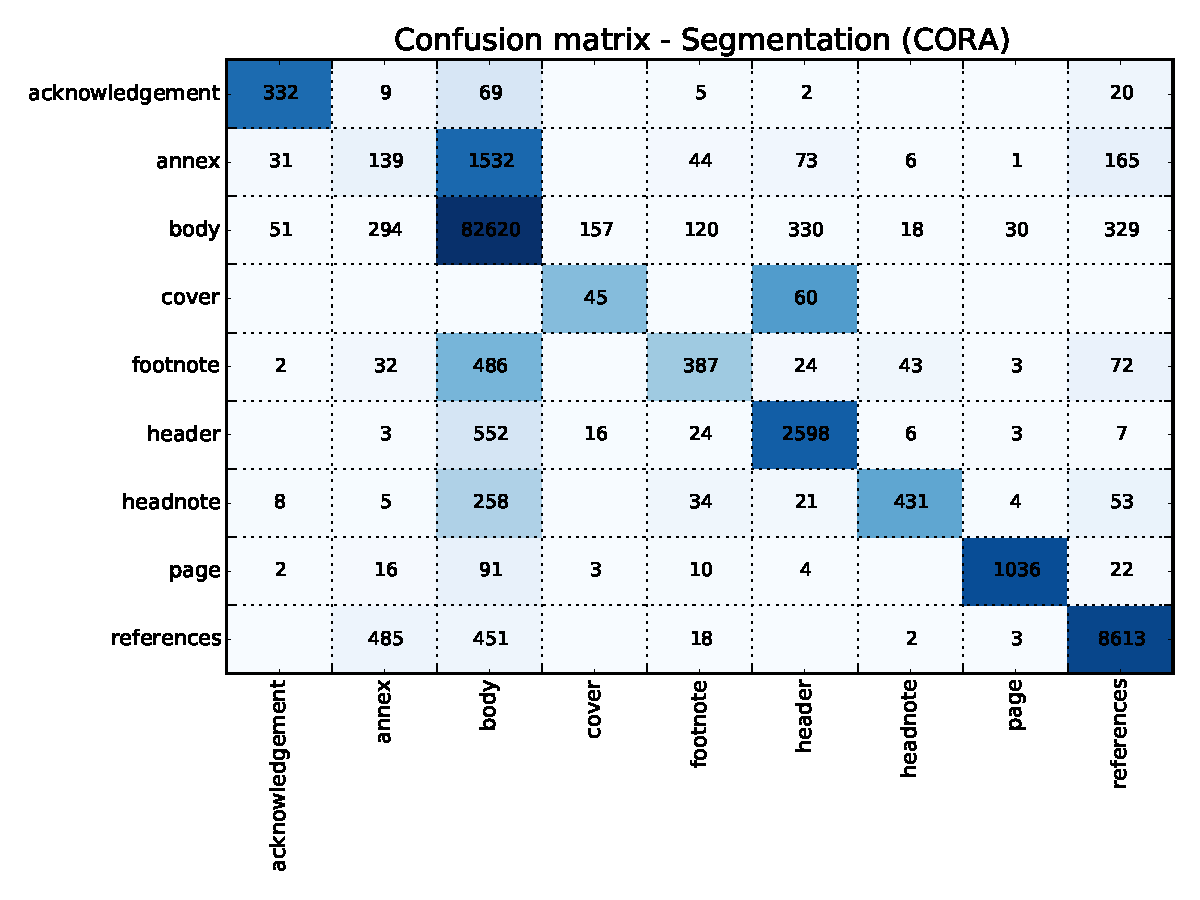
\includegraphics[width=0.75\textwidth]{../../figs/baseline/S_C/confusion_totals.pdf}}
% \end{figure}

% %%%%%%%%%%%%%%%%%%%%%%%%%%%%%%%%%%%%%%%%%%%%%%

% \subsubsection{Segmentation model - Cora dataset appending HEP dataset}

% %%%%%%%%%%%%%%%%%%%%%%%%%%%%%%%%%%%%%%%%%%%%%%

% \begin{figure}[H]
%   \centering
%   \subfloat[][]{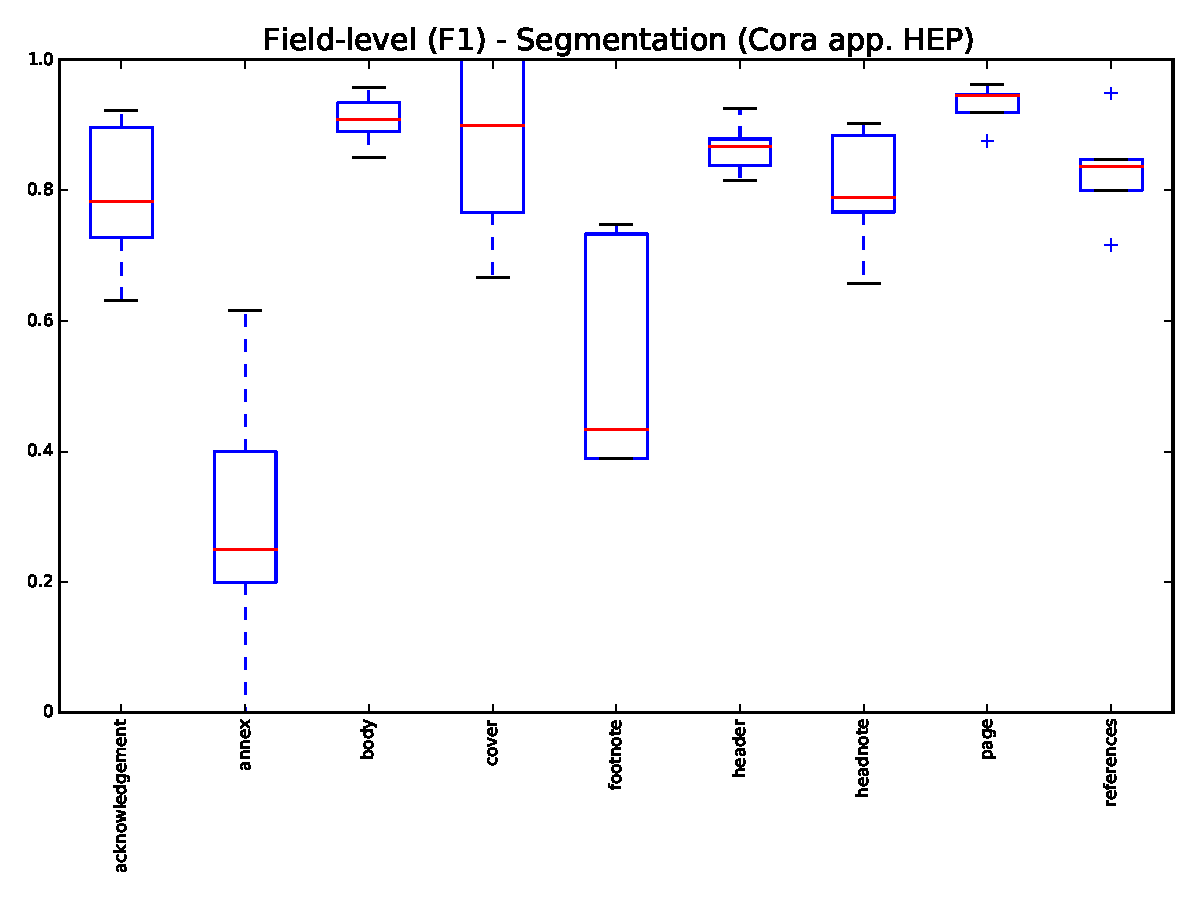
\includegraphics[width=0.75\textwidth]{../../figs/baseline/S_CappH/boxplot-field-level.pdf}}\\
%   \subfloat[][]{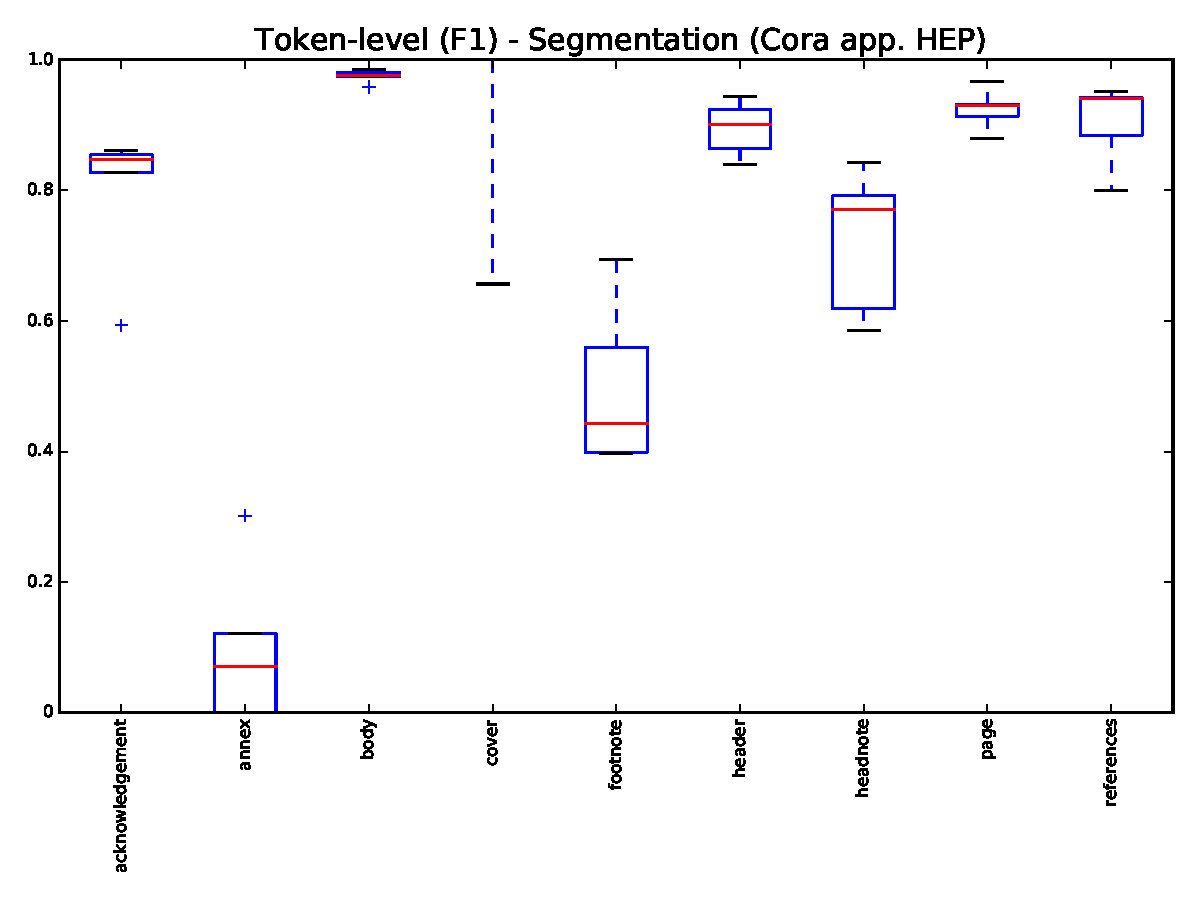
\includegraphics[width=0.75\textwidth]{../../figs/baseline/S_CappH/boxplot-token-level.pdf}}
% \end{figure}

% \begin{figure}[H]
%   \centering
%   \subfloat[][]{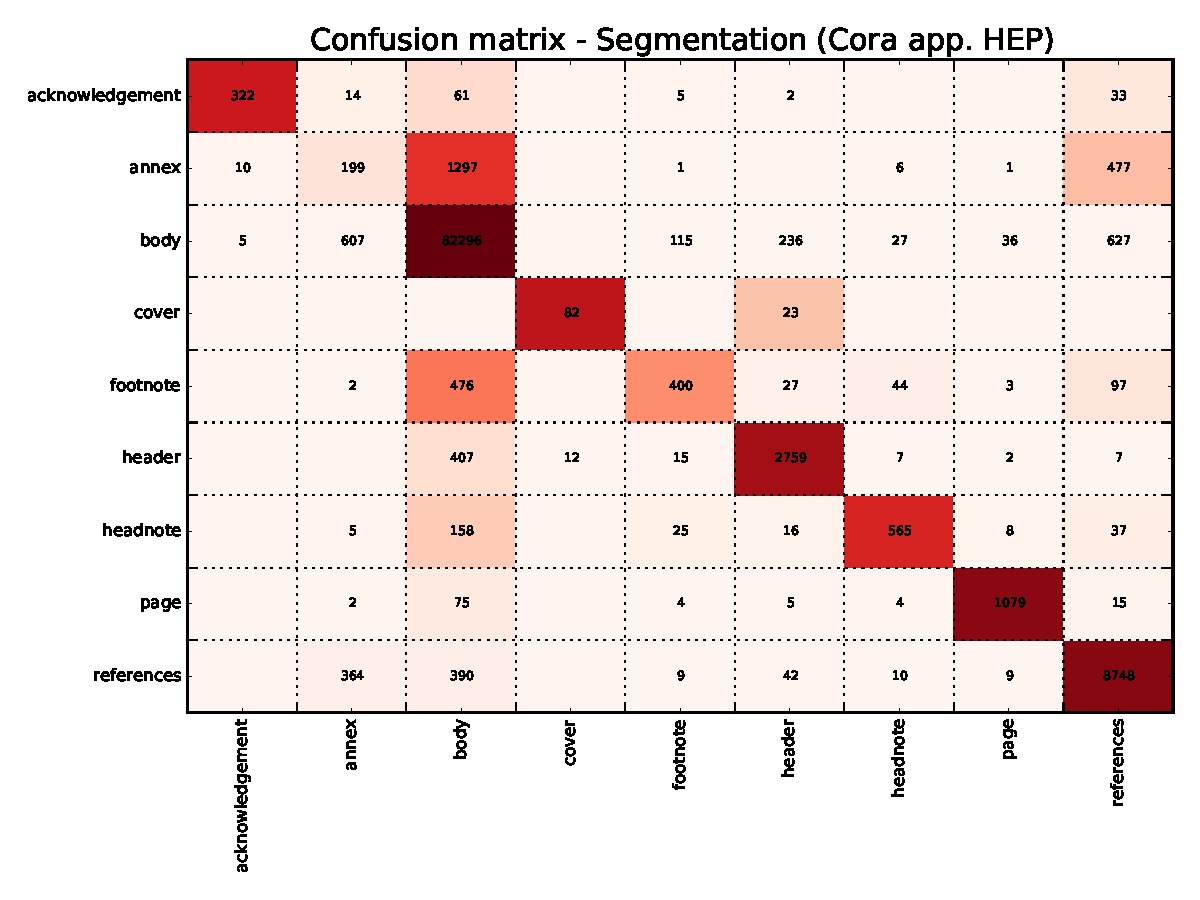
\includegraphics[width=0.75\textwidth]{../../figs/baseline/S_CappH/confusion_totals.pdf}}
% \end{figure}

% %%%%%%%%%%%%%%%%%%%%%%%%%%%%%%%%%%%%%%%%%%%%%%

% \subsubsection{Segmentation model - Cora and HEP combined datasets}

% %%%%%%%%%%%%%%%%%%%%%%%%%%%%%%%%%%%%%%%%%%%%%%

% \begin{figure}[H]
%   \centering
%   \subfloat[][]{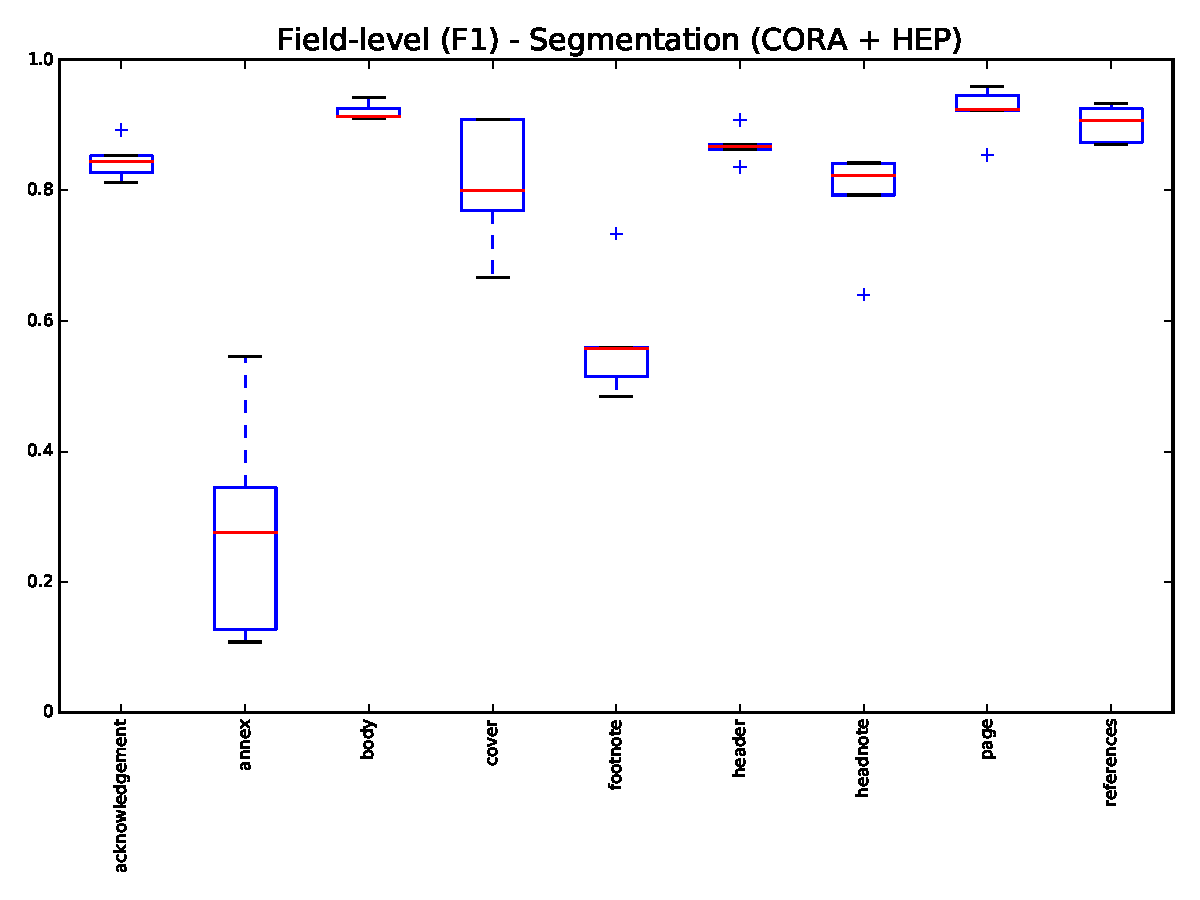
\includegraphics[width=0.75\textwidth]{../../figs/baseline/S_CH/boxplot-field-level.pdf}}\\
%   \subfloat[][]{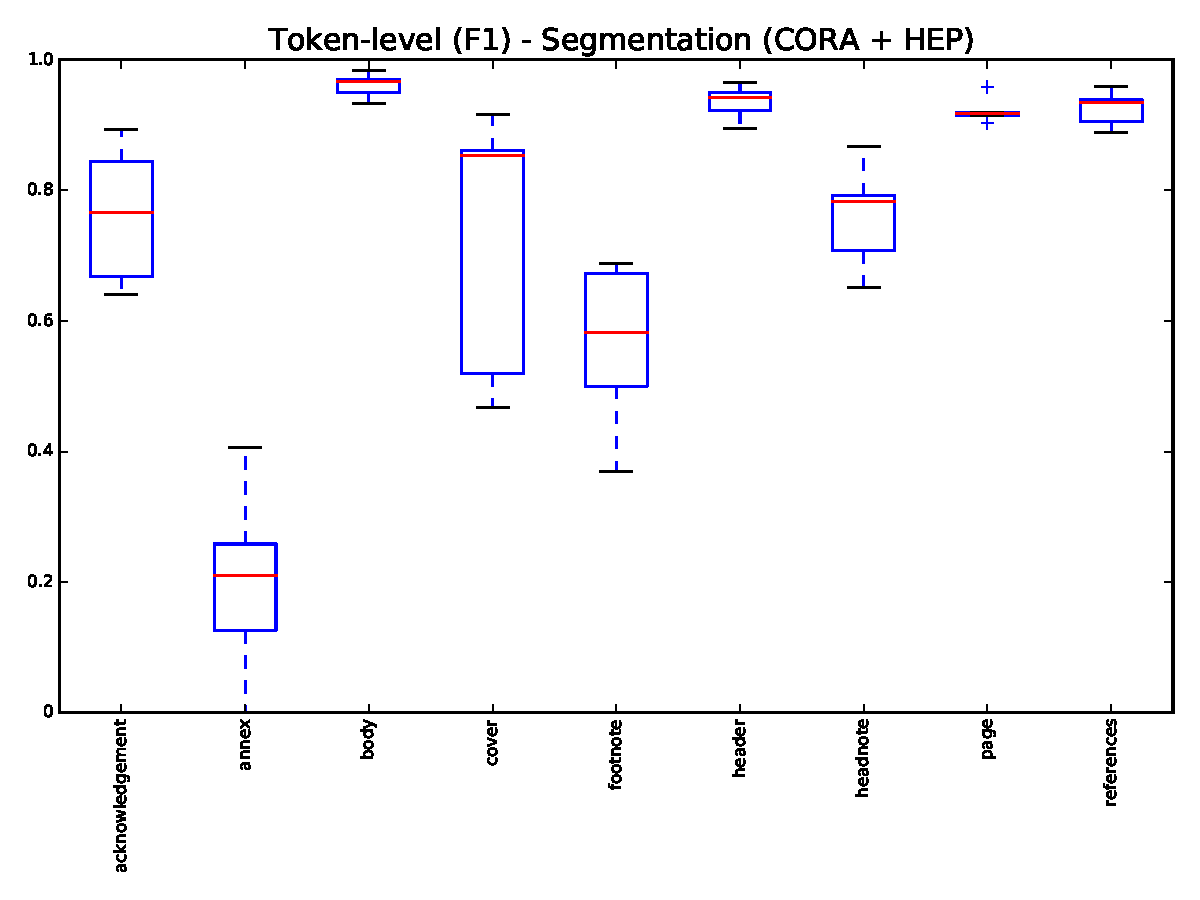
\includegraphics[width=0.75\textwidth]{../../figs/baseline/S_CH/boxplot-token-level.pdf}}
% \end{figure}

% \begin{figure}[H]
%   \centering
%   \subfloat[][]{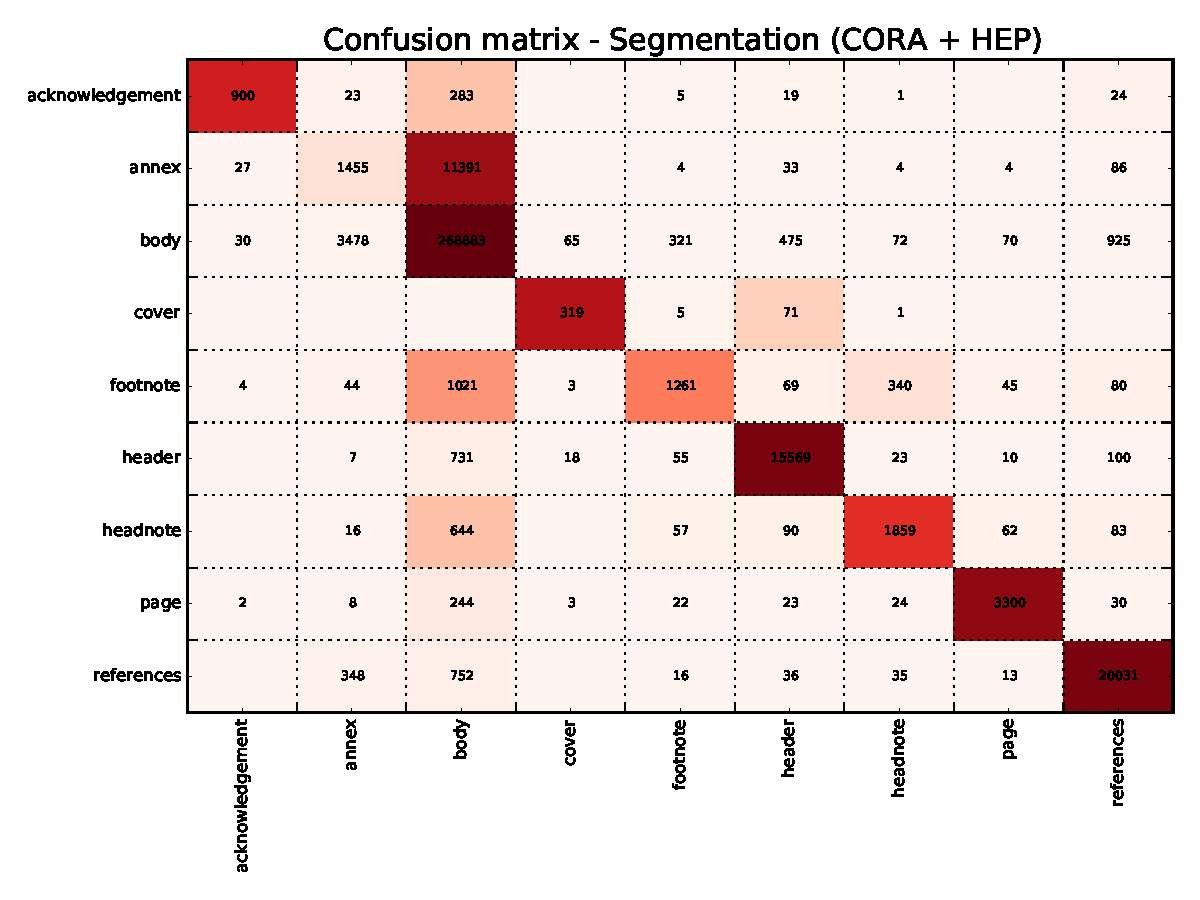
\includegraphics[width=0.75\textwidth]{../../figs/baseline/S_CH/confusion_totals.pdf}}
% \end{figure}

% %%%%%%%%%%%%%%%%%%%%%%%%%%%%%%%%%%%%%%%%%%%%%%

% \subsubsection{Segmentation model - HEP dataset}

% %%%%%%%%%%%%%%%%%%%%%%%%%%%%%%%%%%%%%%%%%%%%%%

% \begin{figure}[H]
%   \centering
%   \subfloat[][]{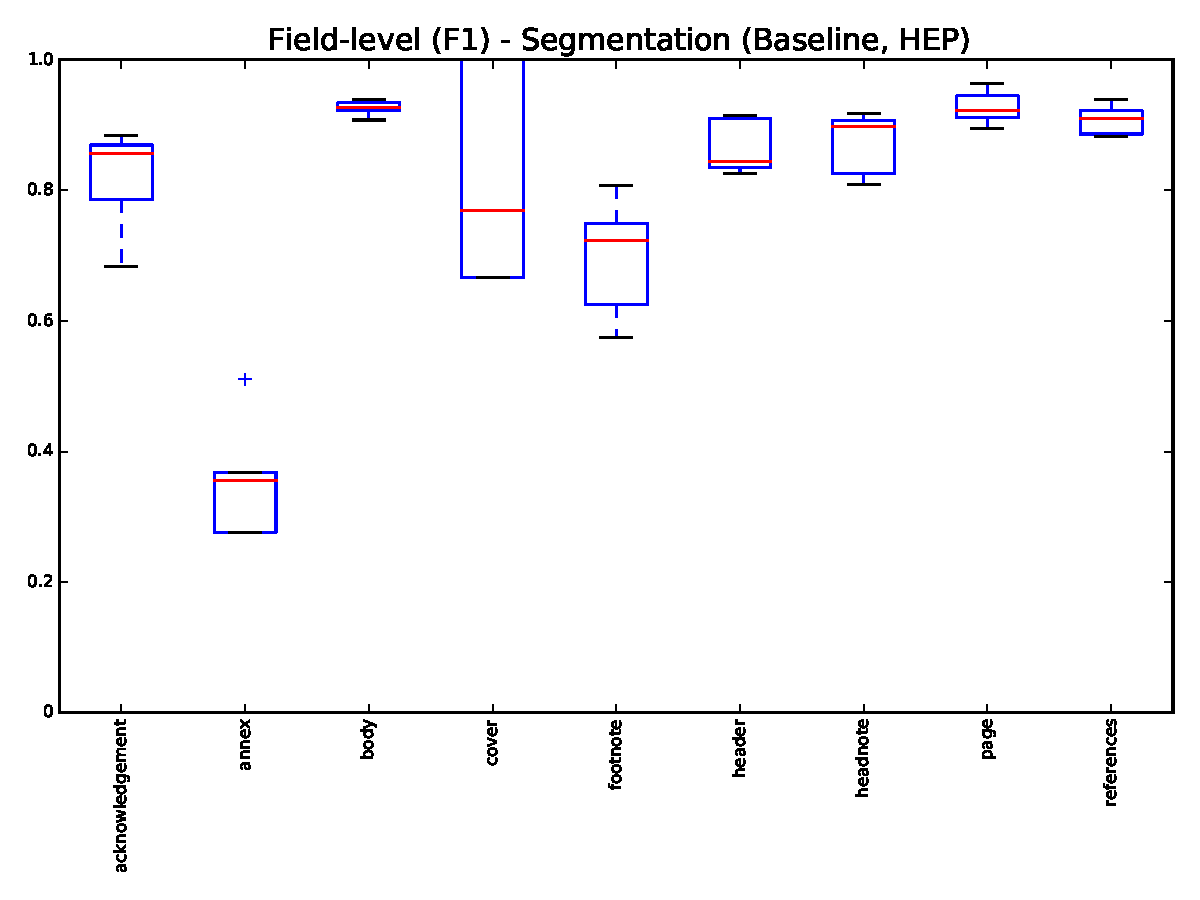
\includegraphics[width=0.75\textwidth]{../../figs/baseline/S_H/boxplot-field-level.pdf}}\\
%   \subfloat[][]{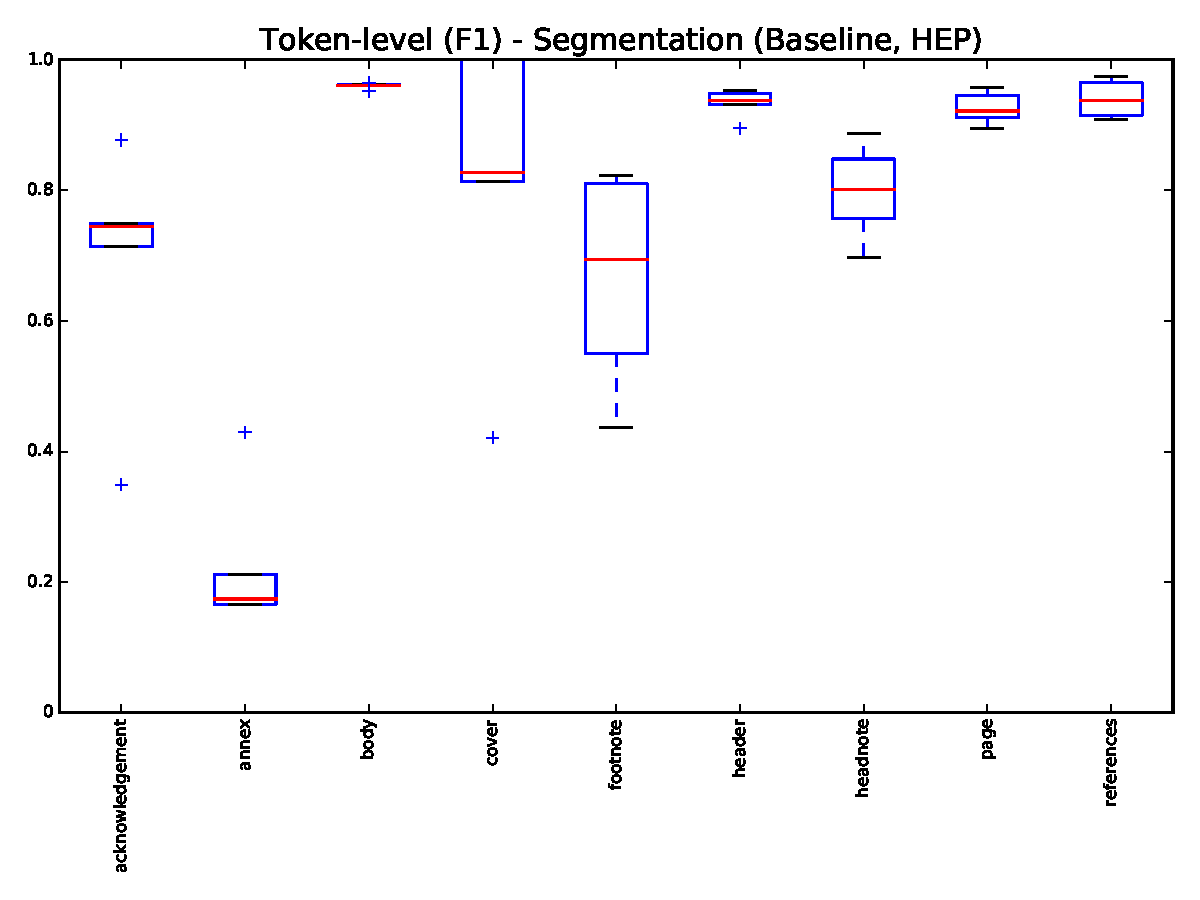
\includegraphics[width=0.75\textwidth]{../../figs/baseline/S_H/boxplot-token-level.pdf}}
% \end{figure}

% \begin{figure}[H]
%   \centering
%   \subfloat[][]{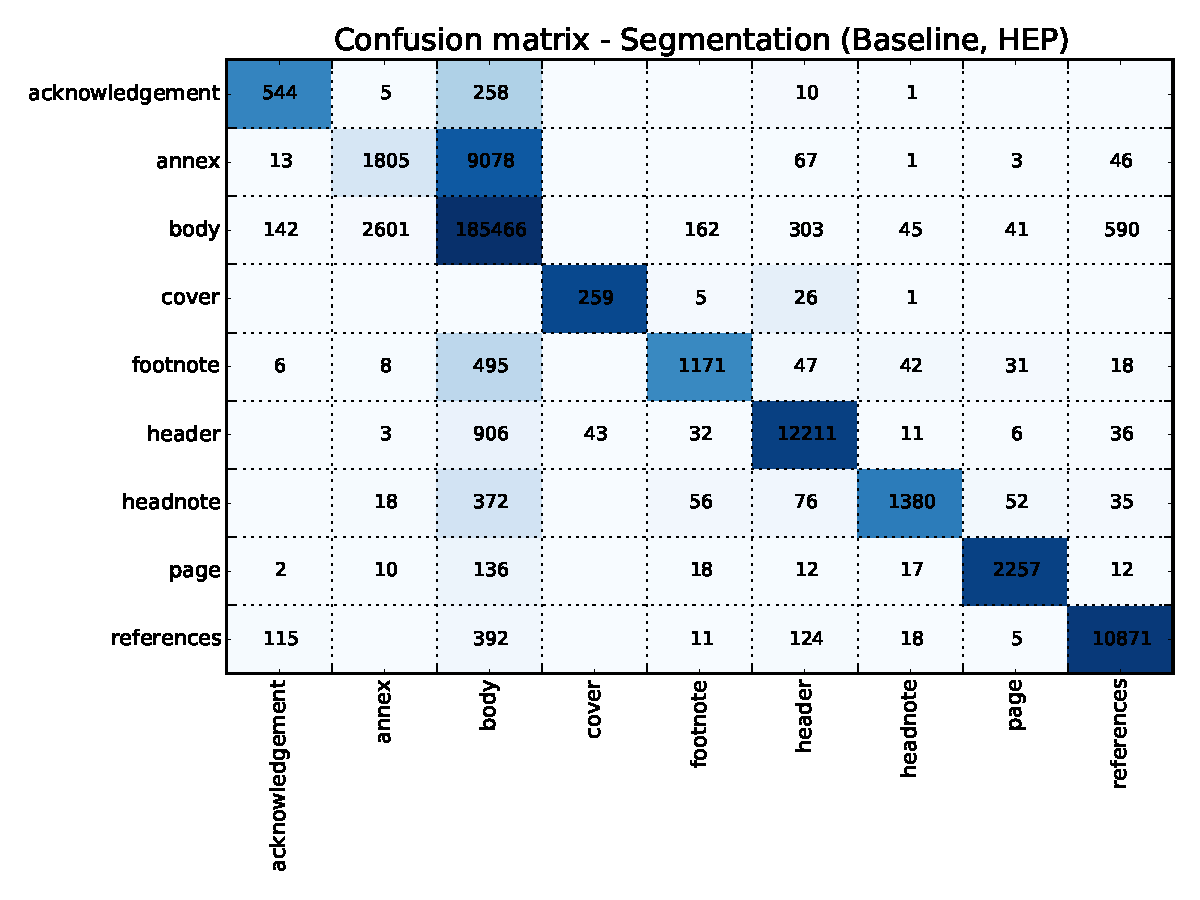
\includegraphics[width=0.75\textwidth]{../../figs/baseline/S_H/confusion_totals.pdf}}
% \end{figure}

% %%%%%%%%%%%%%%%%%%%%%%%%%%%%%%%%%%%%%%%%%%%%%%

% \subsubsection{Segmentation model - HEP dataset appending CORA dataset}

% %%%%%%%%%%%%%%%%%%%%%%%%%%%%%%%%%%%%%%%%%%%%%%

% \begin{figure}[H]
%   \centering
%   \subfloat[][]{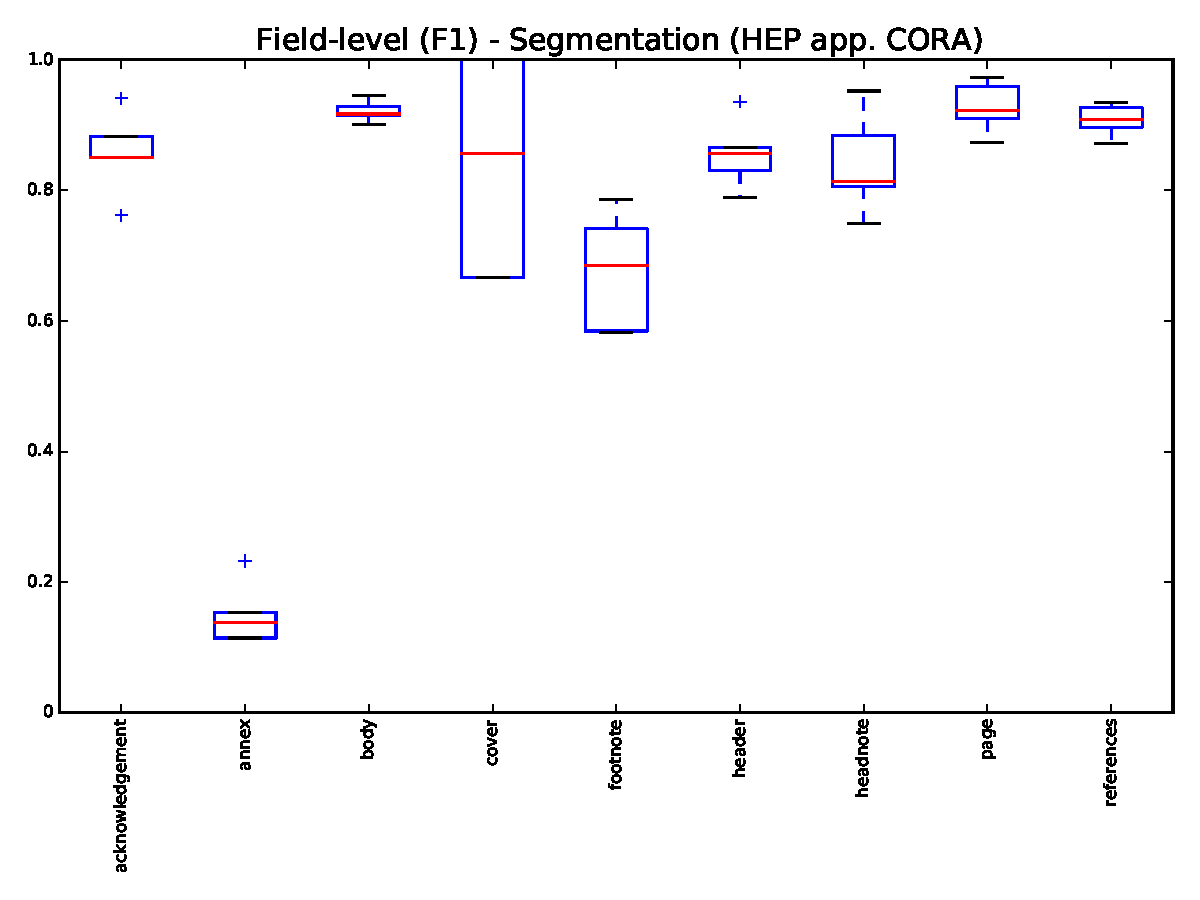
\includegraphics[width=0.75\textwidth]{../../figs/baseline/S_HappC/boxplot-field-level.pdf}}\\
%   \subfloat[][]{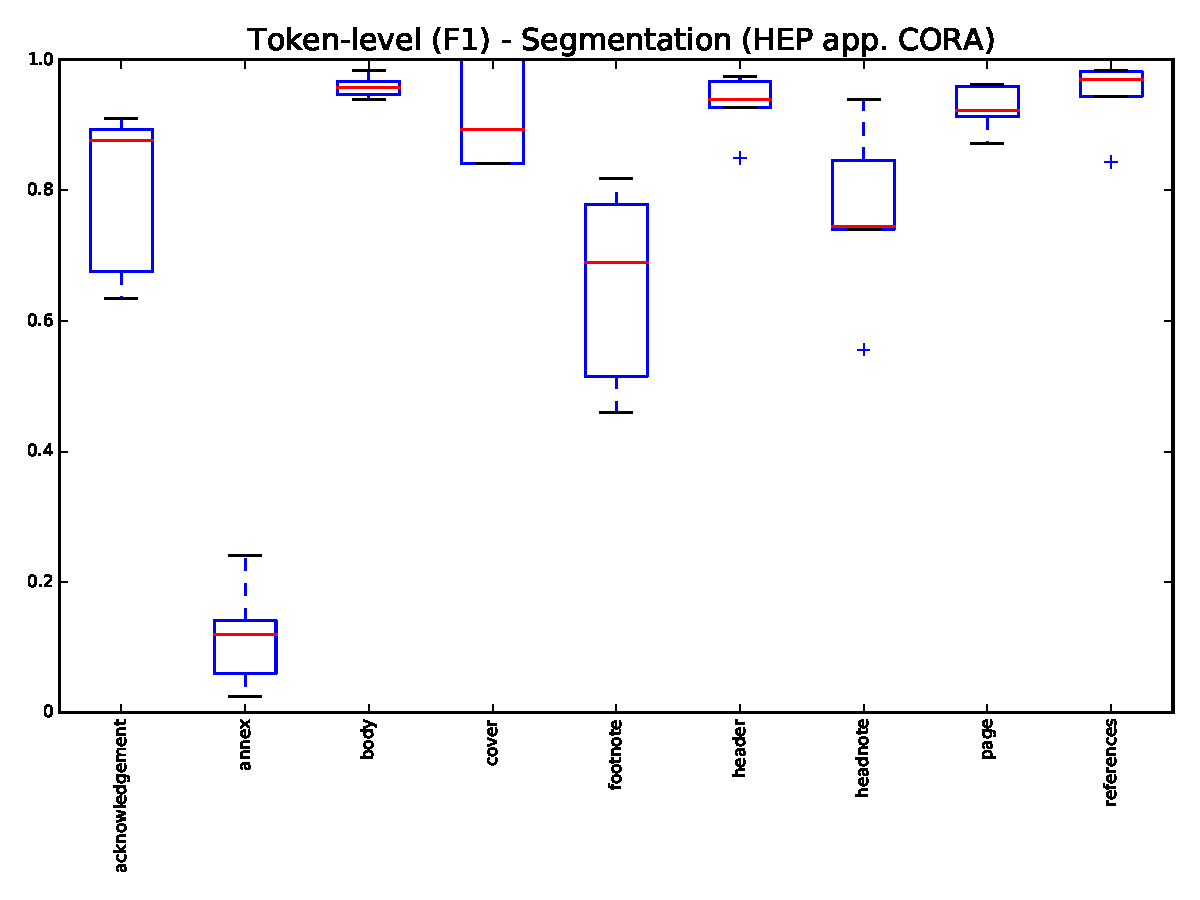
\includegraphics[width=0.75\textwidth]{../../figs/baseline/S_HappC/boxplot-token-level.pdf}}
% \end{figure}

% \begin{figure}[H]
%   \centering
%   \subfloat[][]{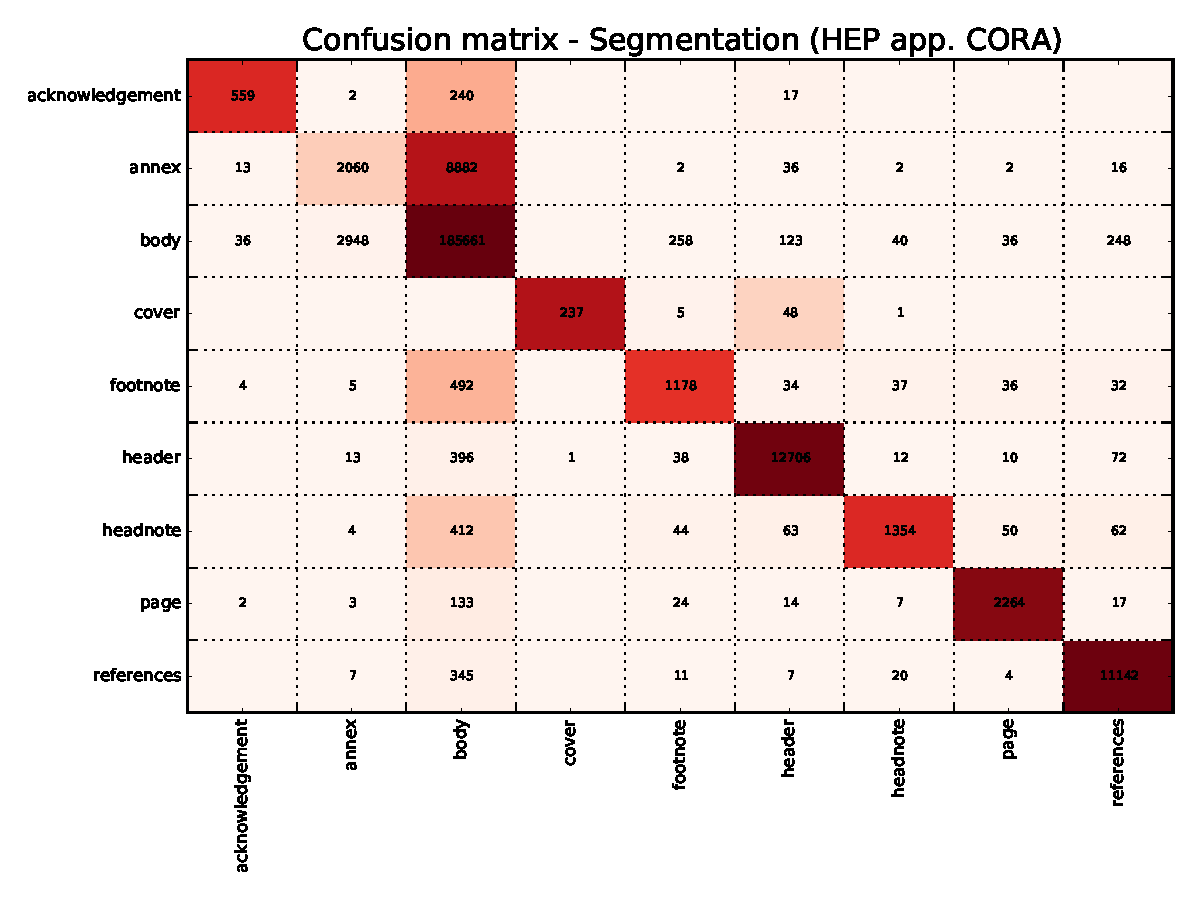
\includegraphics[width=0.75\textwidth]{../../figs/baseline/S_HappC/confusion_totals.pdf}}
% \end{figure}

% %%%%%%%%%%%%%%%%%%%%%%%%%%%%%%%%%%%%%%%%%%%%%%

% \subsection{Regularisation}
% \subsubsection{Header model - $L2 = 0$}

% %%%%%%%%%%%%%%%%%%%%%%%%%%%%%%%%%%%%%%%%%%%%%%

% \begin{figure}[H]
%   \centering
%   \subfloat[][]{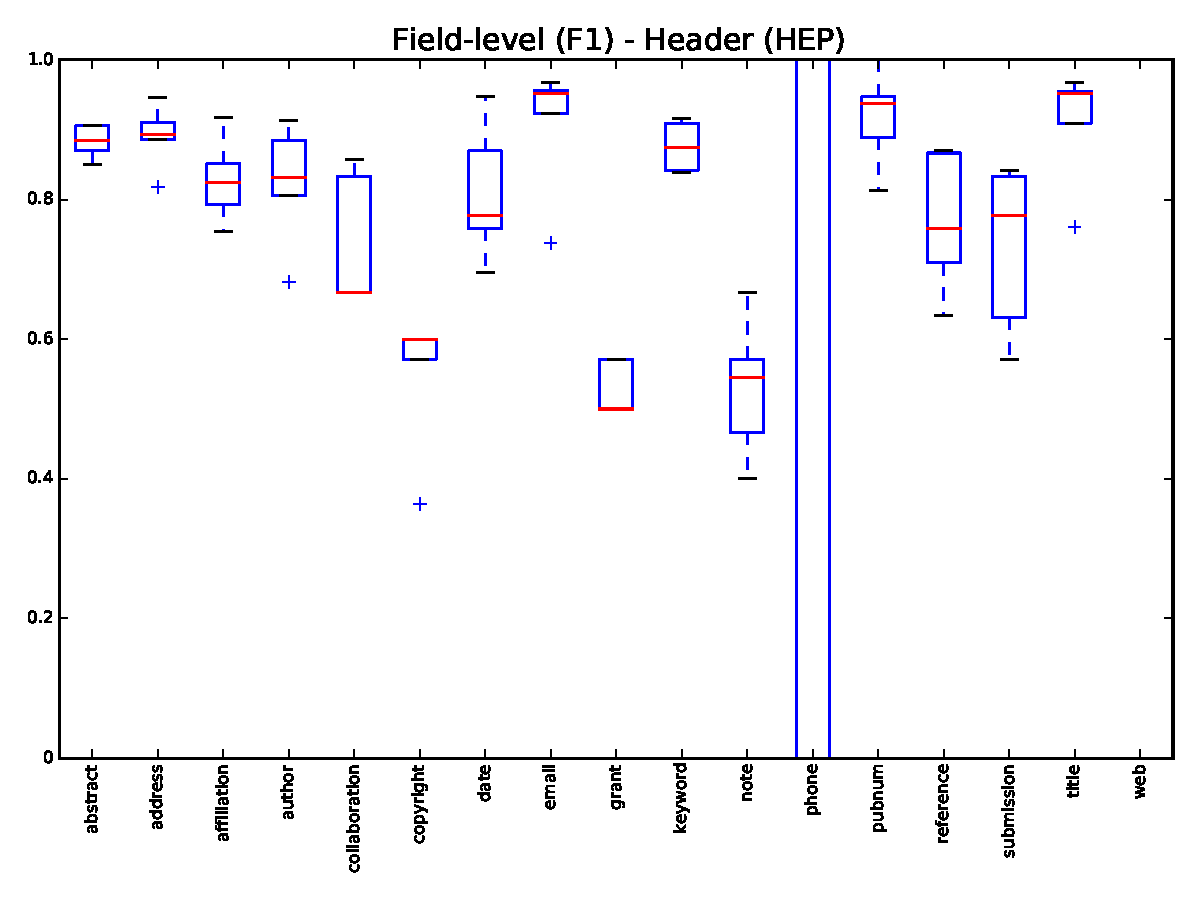
\includegraphics[width=0.75\textwidth]{../../figs/regularisation/H_H_L20/boxplot-field-level.pdf}}\\
%   \subfloat[][]{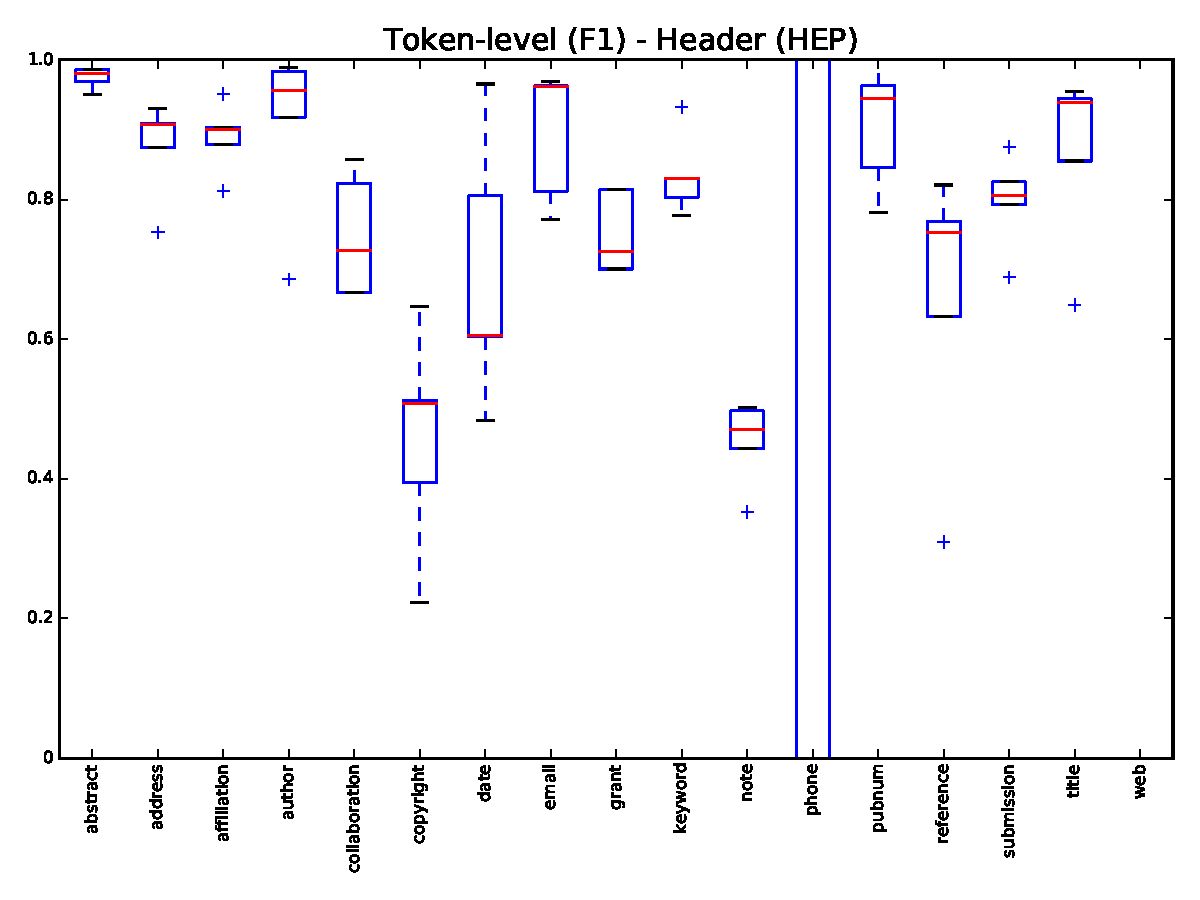
\includegraphics[width=0.75\textwidth]{../../figs/regularisation/H_H_L20/boxplot-token-level.pdf}}
% \end{figure}

% \begin{figure}[H]
%   \centering
%   \subfloat[][]{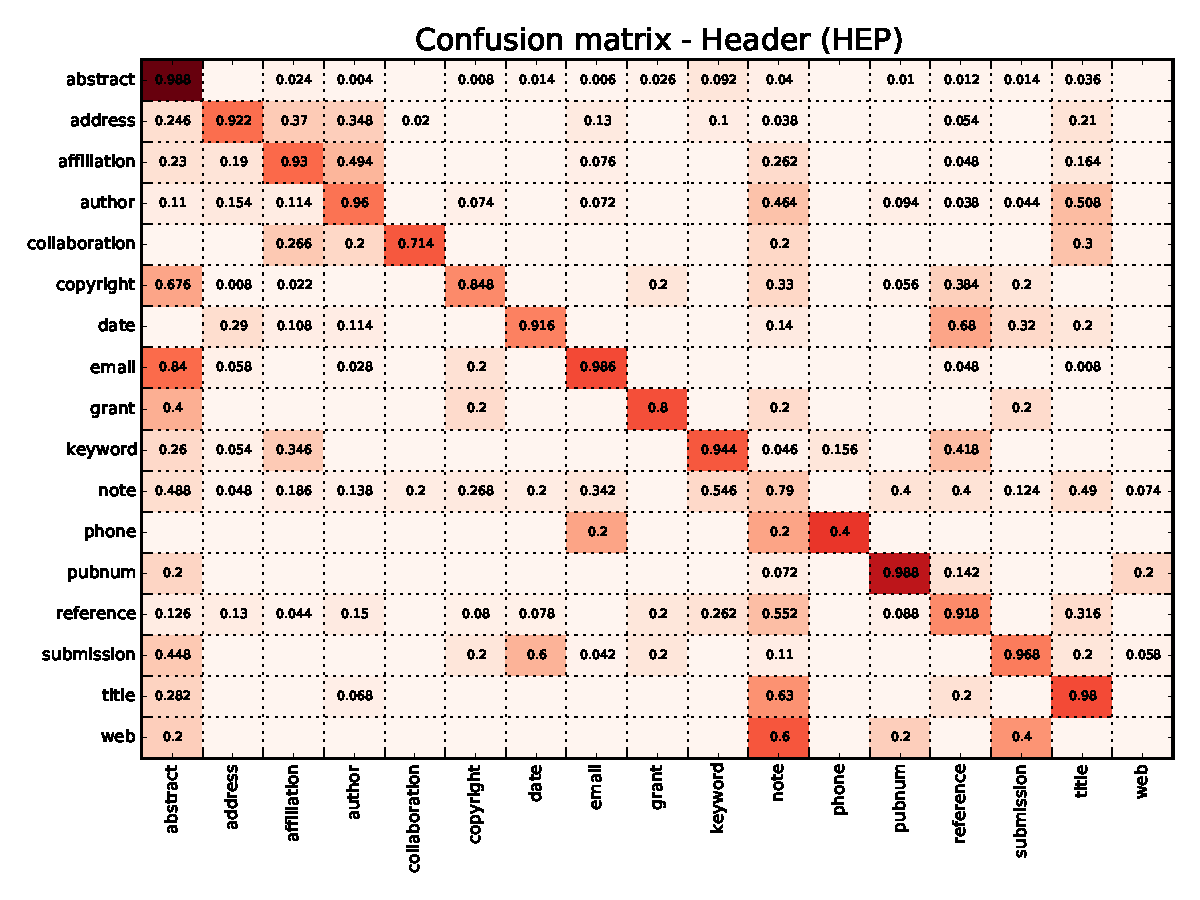
\includegraphics[width=0.75\textwidth]{../../figs/regularisation/H_H_L20/confusion_averages.pdf}}\\
%   \subfloat[][]{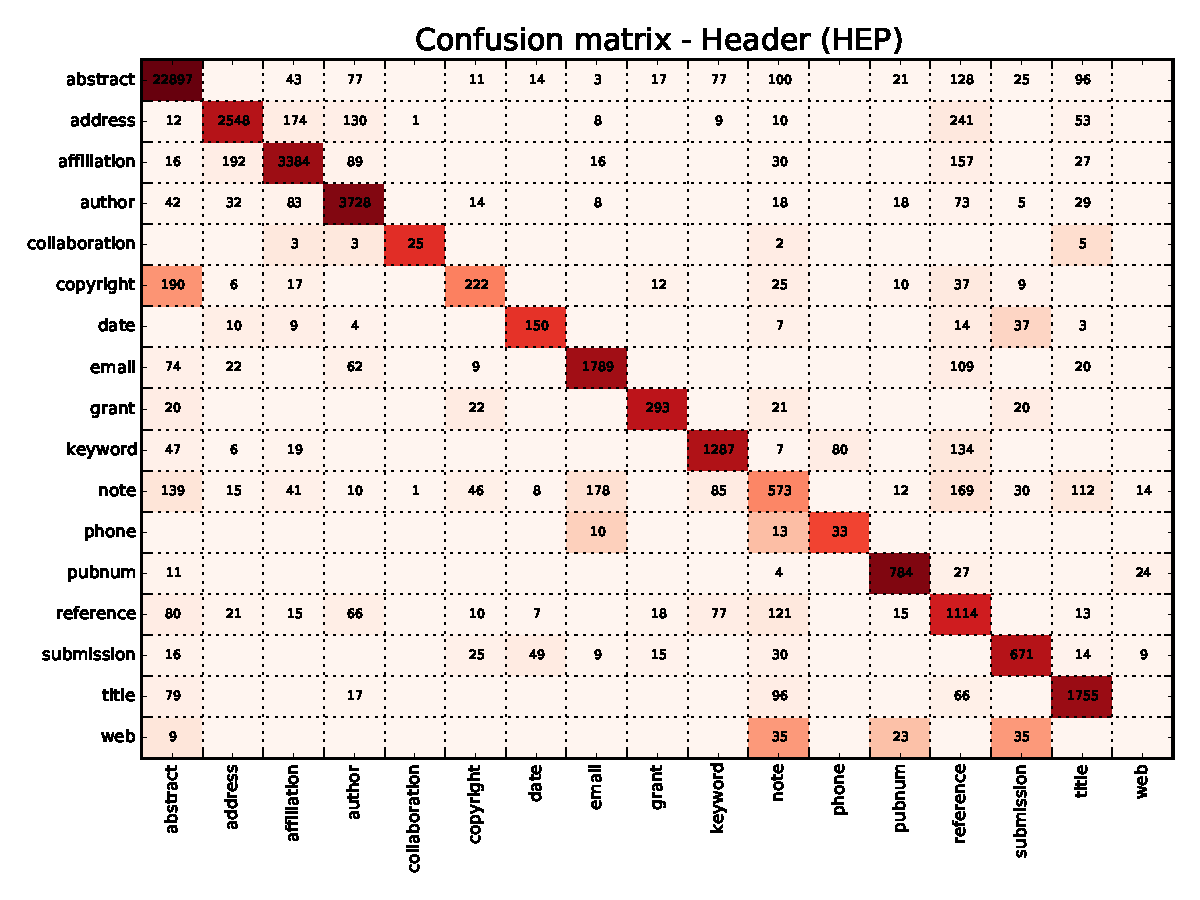
\includegraphics[width=0.75\textwidth]{../../figs/regularisation/H_H_L20/confusion_totals.pdf}}
% \end{figure}

% %%%%%%%%%%%%%%%%%%%%%%%%%%%%%%%%%%%%%%%%%%%%%%

% \subsubsection{Header model - $L2 = 1e^{-6}$}

% %%%%%%%%%%%%%%%%%%%%%%%%%%%%%%%%%%%%%%%%%%%%%%

% \begin{figure}[H]
%   \centering
%   \subfloat[][]{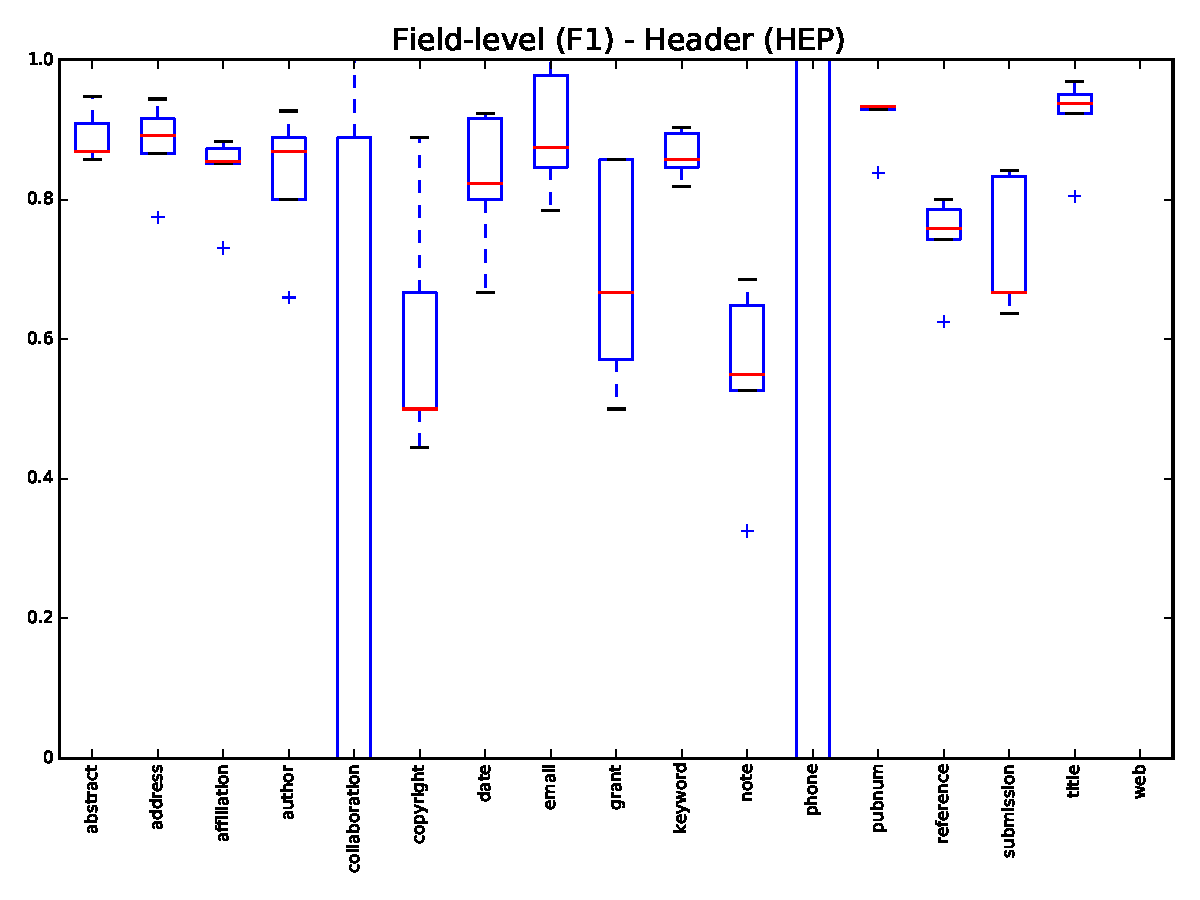
\includegraphics[width=0.75\textwidth]{../../figs/regularisation/H_H_L2e-6/boxplot-field-level.pdf}}\\
%   \subfloat[][]{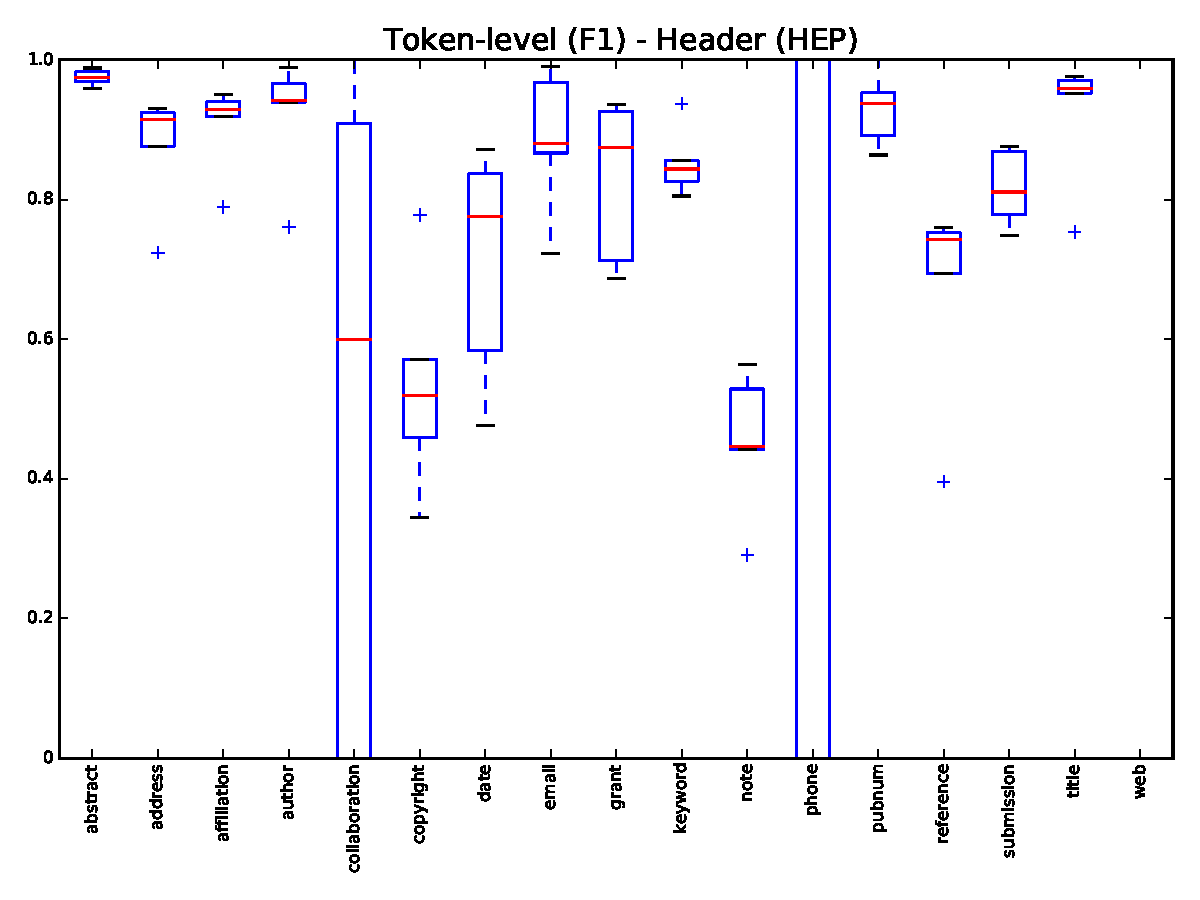
\includegraphics[width=0.75\textwidth]{../../figs/regularisation/H_H_L2e-6/boxplot-token-level.pdf}}
% \end{figure}

% \begin{figure}[H]
%   \centering
%   \subfloat[][]{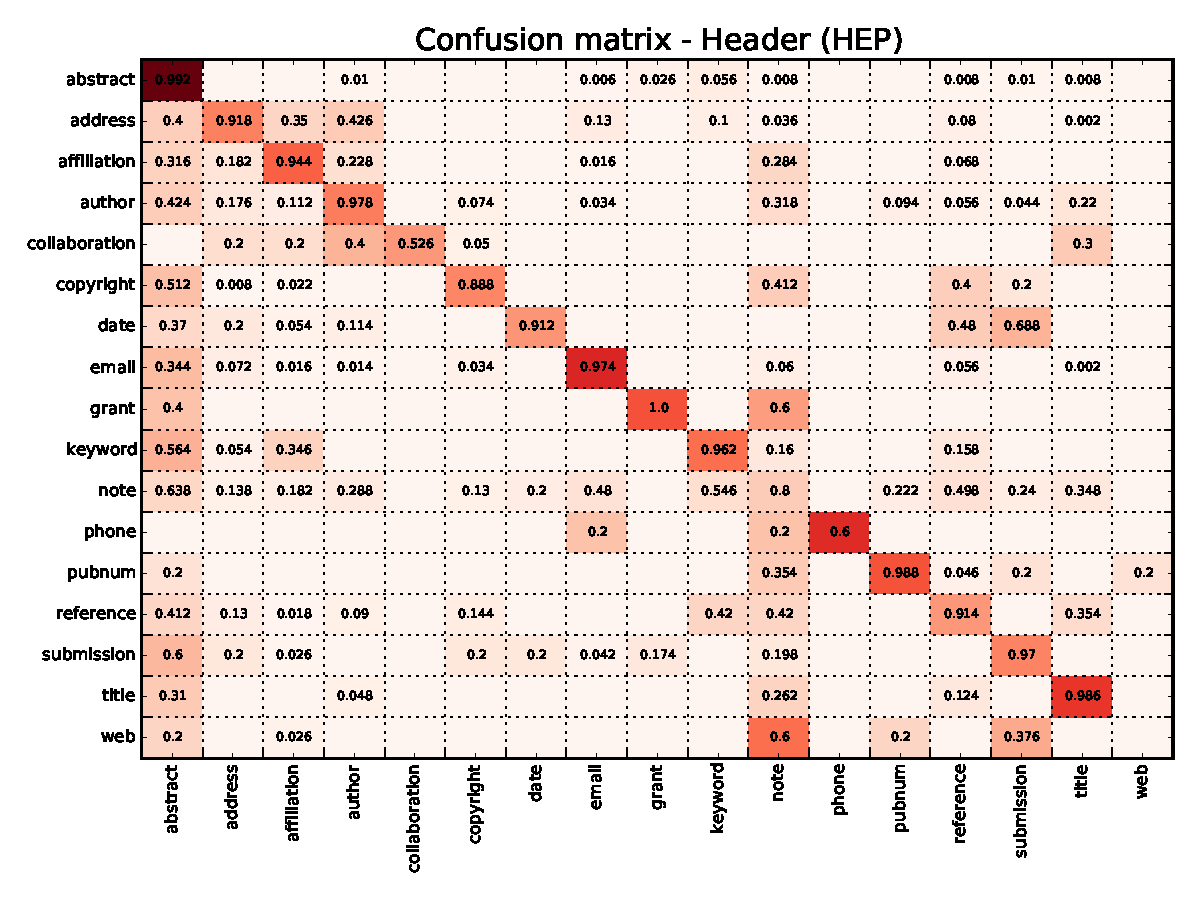
\includegraphics[width=0.75\textwidth]{../../figs/regularisation/H_H_L2e-6/confusion_averages.pdf}}\\
%   \subfloat[][]{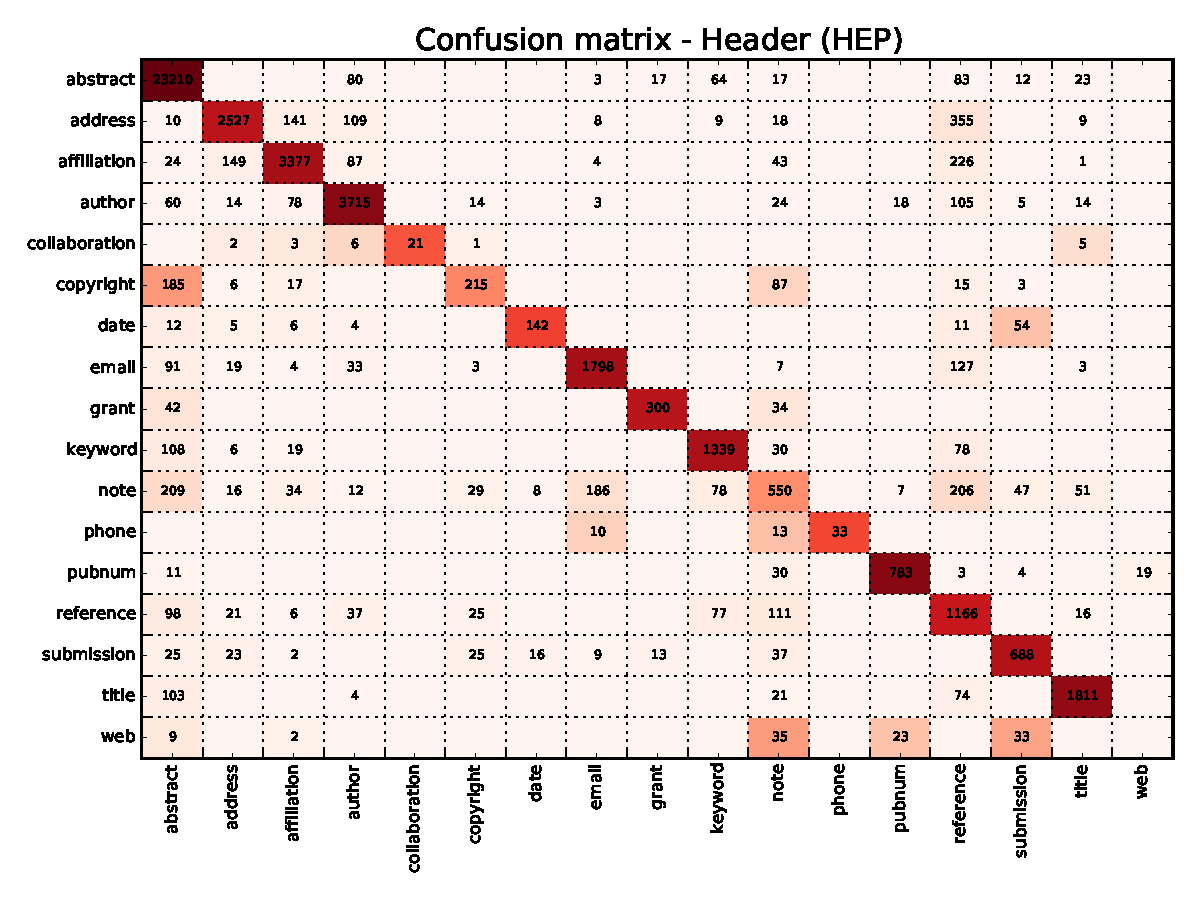
\includegraphics[width=0.75\textwidth]{../../figs/regularisation/H_H_L2e-6/confusion_totals.pdf}}
% \end{figure}

% %%%%%%%%%%%%%%%%%%%%%%%%%%%%%%%%%%%%%%%%%%%%%%

% \subsubsection{Header model - $L2 = 1e^{-5}$}

% %%%%%%%%%%%%%%%%%%%%%%%%%%%%%%%%%%%%%%%%%%%%%%

% \begin{figure}[H]
%   \centering
%   \subfloat[][]{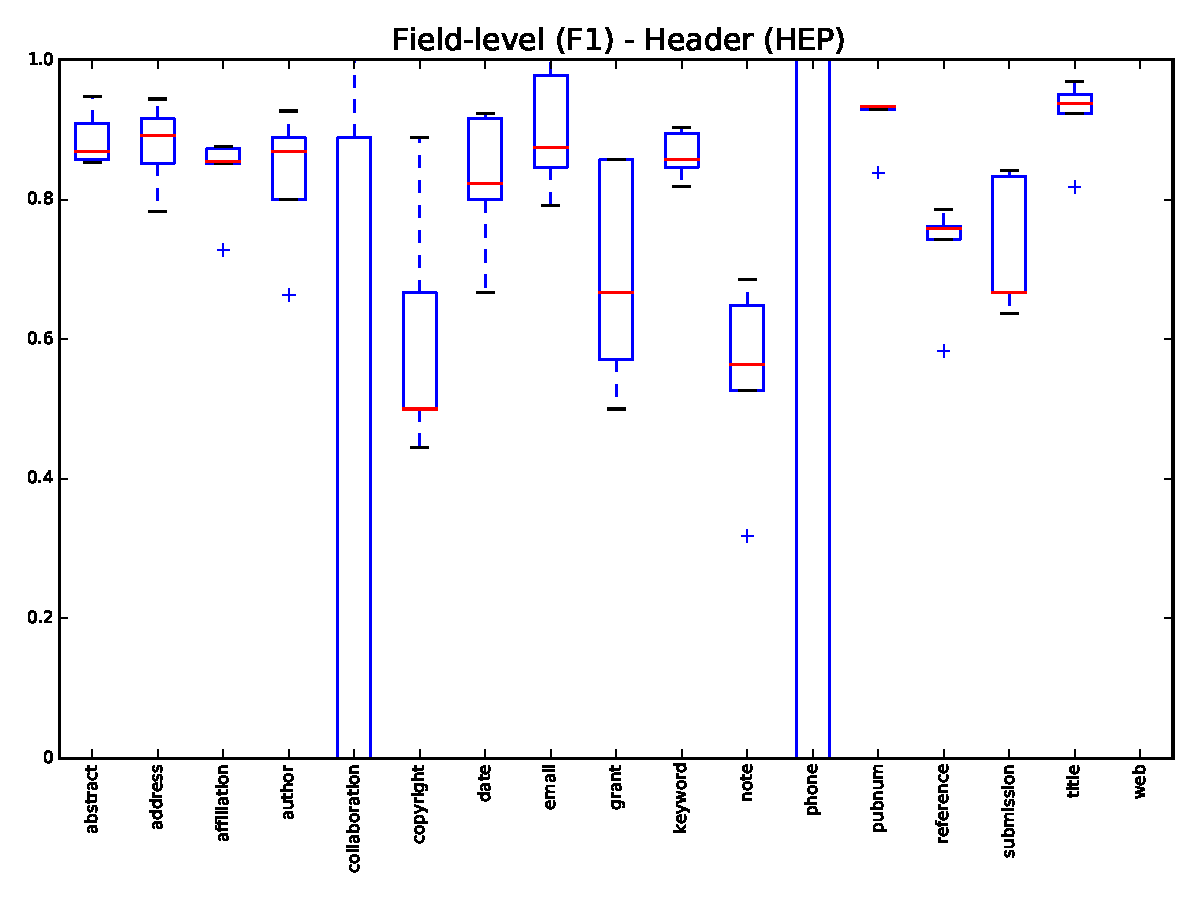
\includegraphics[width=0.75\textwidth]{../../figs/regularisation/H_H_L2e-5/boxplot-field-level.pdf}}\\
%   \subfloat[][]{\includegraphics[width=0.75\textwidth]{../../figs/regularisation/H_H_L2e-5/boxplot-token-level.pdf}}
% \end{figure}

% \begin{figure}[H]
%   \centering
%   \subfloat[][]{\includegraphics[width=0.75\textwidth]{../../figs/regularisation/H_H_L2e-5/confusion_averages.pdf}}\\
%   \subfloat[][]{\includegraphics[width=0.75\textwidth]{../../figs/regularisation/H_H_L2e-5/confusion_totals.pdf}}
% \end{figure}

% %%%%%%%%%%%%%%%%%%%%%%%%%%%%%%%%%%%%%%%%%%%%%%

% \subsubsection{Header model - $L2 = 1e^{-4}$}

% %%%%%%%%%%%%%%%%%%%%%%%%%%%%%%%%%%%%%%%%%%%%%%

% \begin{figure}[H]
%   \centering
%   \subfloat[][]{\includegraphics[width=0.75\textwidth]{../../figs/regularisation/H_H_L2e-4/boxplot-field-level.pdf}}\\
%   \subfloat[][]{\includegraphics[width=0.75\textwidth]{../../figs/regularisation/H_H_L2e-4/boxplot-token-level.pdf}}
% \end{figure}

% \begin{figure}[H]
%   \centering
%   \subfloat[][]{\includegraphics[width=0.75\textwidth]{../../figs/regularisation/H_H_L2e-4/confusion_averages.pdf}}\\
%   \subfloat[][]{\includegraphics[width=0.75\textwidth]{../../figs/regularisation/H_H_L2e-4/confusion_totals.pdf}}
% \end{figure}

% %%%%%%%%%%%%%%%%%%%%%%%%%%%%%%%%%%%%%%%%%%%%%%

% \subsubsection{Header model - $L2 = 1e^{-3}$}

% %%%%%%%%%%%%%%%%%%%%%%%%%%%%%%%%%%%%%%%%%%%%%%

% \begin{figure}[H]
%   \centering
%   \subfloat[][]{\includegraphics[width=0.75\textwidth]{../../figs/regularisation/H_H_L2e-3/boxplot-field-level.pdf}}\\
%   \subfloat[][]{\includegraphics[width=0.75\textwidth]{../../figs/regularisation/H_H_L2e-3/boxplot-token-level.pdf}}
% \end{figure}

% \begin{figure}[H]
%   \centering
%   \subfloat[][]{\includegraphics[width=0.75\textwidth]{../../figs/regularisation/H_H_L2e-3/confusion_averages.pdf}}\\
%   \subfloat[][]{\includegraphics[width=0.75\textwidth]{../../figs/regularisation/H_H_L2e-3/confusion_totals.pdf}}
% \end{figure}

% %%%%%%%%%%%%%%%%%%%%%%%%%%%%%%%%%%%%%%%%%%%%%%

% \subsection{Dictionaries}
% \subsubsection{Header model - HEP dataset}

% %%%%%%%%%%%%%%%%%%%%%%%%%%%%%%%%%%%%%%%%%%%%%%

% \begin{figure}[H]
%   \centering
%   \subfloat[][]{\includegraphics[width=0.75\textwidth]{../../figs/dicts/H_H_dicts/boxplot-field-level.pdf}}\\
%   \subfloat[][]{\includegraphics[width=0.75\textwidth]{../../figs/dicts/H_H_dicts/boxplot-token-level.pdf}}
% \end{figure}

% \begin{figure}[H]
%   \centering
%   \subfloat[][]{\includegraphics[width=0.75\textwidth]{../../figs/dicts/H_H_dicts/confusion_averages.pdf}}\\
%   \subfloat[][]{\includegraphics[width=0.75\textwidth]{../../figs/dicts/H_H_dicts/confusion_totals.pdf}}
% \end{figure}

% %%%%%%%%%%%%%%%%%%%%%%%%%%%%%%%%%%%%%%%%%%%%%%

% \subsubsection{Header model - HEP dataset appending CORA dataset}

% %%%%%%%%%%%%%%%%%%%%%%%%%%%%%%%%%%%%%%%%%%%%%%

% \begin{figure}[H]
%   \centering
%   \subfloat[][]{\includegraphics[width=0.75\textwidth]{../../figs/dicts/H_HappC_dicts/boxplot-field-level.pdf}}\\
%   \subfloat[][]{\includegraphics[width=0.75\textwidth]{../../figs/dicts/H_HappC_dicts/boxplot-token-level.pdf}}
% \end{figure}

% \begin{figure}[H]
%   \centering
%   \subfloat[][]{\includegraphics[width=0.75\textwidth]{../../figs/dicts/H_HappC_dicts/confusion_averages.pdf}}\\
%   \subfloat[][]{\includegraphics[width=0.75\textwidth]{../../figs/dicts/H_HappC_dicts/confusion_totals.pdf}}
% \end{figure}

% %%%%%%%%%%%%%%%%%%%%%%%%%%%%%%%%%%%%%%%%%%%%%%

% \subsubsection{Segmentation model - HEP dataset}

% %%%%%%%%%%%%%%%%%%%%%%%%%%%%%%%%%%%%%%%%%%%%%%

% \begin{figure}[H]
%   \centering
%   \subfloat[][]{\includegraphics[width=0.75\textwidth]{../../figs/dicts/S_H_dicts/boxplot-field-level.pdf}}\\
%   \subfloat[][]{\includegraphics[width=0.75\textwidth]{../../figs/dicts/S_H_dicts/boxplot-token-level.pdf}}
% \end{figure}

% \begin{figure}[H]
%   \centering
%   \subfloat[][]{\includegraphics[width=0.75\textwidth]{../../figs/dicts/S_H_dicts/confusion_averages.pdf}}\\
%   \subfloat[][]{\includegraphics[width=0.75\textwidth]{../../figs/dicts/S_H_dicts/confusion_totals.pdf}}
% \end{figure}

% %%%%%%%%%%%%%%%%%%%%%%%%%%%%%%%%%%%%%%%%%%%%%%

% \subsubsection{Segmentation model - HEP dataset appending CORA dataset}

% %%%%%%%%%%%%%%%%%%%%%%%%%%%%%%%%%%%%%%%%%%%%%%

% \begin{figure}[H]
%   \centering
%   \subfloat[][]{\includegraphics[width=0.75\textwidth]{../../figs/dicts/S_HappC_dicts/boxplot-field-level.pdf}}\\
%   \subfloat[][]{\includegraphics[width=0.75\textwidth]{../../figs/dicts/S_HappC_dicts/boxplot-token-level.pdf}}
% \end{figure}

% \begin{figure}[H]
%   \centering
%   \subfloat[][]{\includegraphics[width=0.75\textwidth]{../../figs/dicts/S_HappC_dicts/confusion_averages.pdf}}\\
%   \subfloat[][]{\includegraphics[width=0.75\textwidth]{../../figs/dicts/S_HappC_dicts/confusion_totals.pdf}}
% \end{figure}

% %%%%%%%%%%%%%%%%%%%%%%%%%%%%%%%%%%%%%%%%%%%%%%

% \subsubsection{Header Model - HEP dataset - $2^{nd}$ Degree Features}
% \subsubsection{Header Model - HEP dataset Appending CORA - $2^{nd}$ Degree Features}
% \subsubsection{Header Model - HEP dataset - $3^{rd}$ Degree Features}
% \subsubsection{Header Model - HEP dataset Appending CORA - $3^{rd}$ Degree Features}

% \subsection{Dictionaries + stop words}
% \subsubsection{Header model - HEP dataset}

% %%%%%%%%%%%%%%%%%%%%%%%%%%%%%%%%%%%%%%%%%%%%%%

% \begin{figure}[H]
%   \centering
%   \subfloat[][]{\includegraphics[width=0.75\textwidth]{../../figs/dicts_stops/H_H_dicts_stops/boxplot-field-level.pdf}}\\
%   \subfloat[][]{\includegraphics[width=0.75\textwidth]{../../figs/dicts_stops/H_H_dicts_stops/boxplot-token-level.pdf}}
% \end{figure}

% \begin{figure}[H]
%   \centering
%   \subfloat[][]{\includegraphics[width=0.75\textwidth]{../../figs/dicts_stops/H_H_dicts_stops/confusion_averages.pdf}}\\
%   \subfloat[][]{\includegraphics[width=0.75\textwidth]{../../figs/dicts_stops/H_H_dicts_stops/confusion_totals.pdf}}
% \end{figure}

% %%%%%%%%%%%%%%%%%%%%%%%%%%%%%%%%%%%%%%%%%%%%%%

% \subsubsection{Header model - HEP dataset appending CORA dataset}

% %%%%%%%%%%%%%%%%%%%%%%%%%%%%%%%%%%%%%%%%%%%%%%

% \begin{figure}[H]
%   \centering
%   \subfloat[][]{\includegraphics[width=0.75\textwidth]{../../figs/dicts_stops/H_HappC_dicts_stops/boxplot-field-level.pdf}}\\
%   \subfloat[][]{\includegraphics[width=0.75\textwidth]{../../figs/dicts_stops/H_HappC_dicts_stops/boxplot-token-level.pdf}}
% \end{figure}

% \begin{figure}[H]
%   \centering
%   \subfloat[][]{\includegraphics[width=0.75\textwidth]{../../figs/dicts_stops/H_HappC_dicts_stops/confusion_averages.pdf}}\\
%   \subfloat[][]{\includegraphics[width=0.75\textwidth]{../../figs/dicts_stops/H_HappC_dicts_stops/confusion_totals.pdf}}
% \end{figure}

% %%%%%%%%%%%%%%%%%%%%%%%%%%%%%%%%%%%%%%%%%%%%%%

% \subsubsection{Segmentation model - HEP dataset}

% %%%%%%%%%%%%%%%%%%%%%%%%%%%%%%%%%%%%%%%%%%%%%%

% \begin{figure}[H]
%   \centering
%   \subfloat[][]{\includegraphics[width=0.75\textwidth]{../../figs/dicts_stops/S_H_dicts_stops/boxplot-field-level.pdf}}\\
%   \subfloat[][]{\includegraphics[width=0.75\textwidth]{../../figs/dicts_stops/S_H_dicts_stops/boxplot-token-level.pdf}}
% \end{figure}

% \begin{figure}[H]
%   \centering
%   \subfloat[][]{\includegraphics[width=0.75\textwidth]{../../figs/dicts_stops/S_H_dicts_stops/confusion_averages.pdf}}\\
%   \subfloat[][]{\includegraphics[width=0.75\textwidth]{../../figs/dicts_stops/S_H_dicts_stops/confusion_totals.pdf}}
% \end{figure}

% %%%%%%%%%%%%%%%%%%%%%%%%%%%%%%%%%%%%%%%%%%%%%%

% \subsubsection{Segmentation model - HEP dataset appending CORA dataset}

% %%%%%%%%%%%%%%%%%%%%%%%%%%%%%%%%%%%%%%%%%%%%%%

% \begin{figure}[H]
%   \centering
%   \subfloat[][]{\includegraphics[width=0.75\textwidth]{../../figs/dicts_stops/S_HappC_dicts_stops/boxplot-field-level.pdf}}\\
%   \subfloat[][]{\includegraphics[width=0.75\textwidth]{../../figs/dicts_stops/S_HappC_dicts_stops/boxplot-token-level.pdf}}
% \end{figure}

% \begin{figure}[H]
%   \centering
%   \subfloat[][]{\includegraphics[width=0.75\textwidth]{../../figs/dicts_stops/S_HappC_dicts_stops/confusion_averages.pdf}}\\
%   \subfloat[][]{\includegraphics[width=0.75\textwidth]{../../figs/dicts_stops/S_HappC_dicts_stops/confusion_totals.pdf}}
% \end{figure}

% %%%%%%%%%%%%%%%%%%%%%%%%%%%%%%%%%%%%%%%%%%%%%%

% \subsubsection{Header Model - HEP dataset - $2^{nd}$ Degree Features}
% \subsubsection{Header Model - HEP dataset Appending CORA - $2^{nd}$ Degree Features}
% \subsubsection{Header Model - HEP dataset - $3^{rd}$ Degree Features}
% \subsubsection{Header Model - HEP dataset Appending CORA - $3^{rd}$ Degree Features}

% \subsection{Token Selection}
% \subsubsection{Segmentation Model - HEP dataset - 5 Tokens}
% \subsubsection{Segmentation Model - HEP dataset - 10 Tokens}
% \subsubsection{Segmentation Model - HEP dataset - 15 Tokens}
% \subsubsection{Segmentation Model - HEP dataset - 20 Tokens}

% \subsection{Levenshtein}
% \subsubsection{Segmentation Model - HEP dataset - Binary Threshold (0.05)}
% \subsubsection{Segmentation Model - HEP dataset - Binary Threshold (0.1)}
% \subsubsection{Segmentation Model - HEP dataset - Binary Threshold (0.2)}
% \subsubsection{Segmentation Model - HEP dataset - Binary Threshold (0.4)}
% \subsubsection{Segmentation Model - HEP dataset - Binary Threshold (0.8)}
% \subsubsection{Segmentation Model - HEP dataset - Ternary Threshold}
% \subsubsection{Segmentation Model - HEP dataset - Quaternary Threshold}

% \subsection{Line Shape}
% \subsubsection{Segmentation Model - HEP dataset - Binary Threshold}
% \subsubsection{Segmentation Model - HEP dataset - Ternary Threshold}

% \subsection{Template Matching}
% \subsubsection{Segmentation Model - HEP dataset}

% \section{Conclusion}
% \subsection{Summary}
% \subsubsection{Key Results}
% \subsection{Future Work}

% \section{References}
% % http://dblp.uni-trier.de/

% \section{Appendices}

\end{document}